\section{Esperienza 3}
\subsection{3.1}
In quest'esperienza si valutano vari parametri caratteristici di dispositivi a semiconduttore come diodi, diodi LED e diodi Zener, in particolare se ne valuterà la tensione di soglia, ovvero, la tensione dopo la quale il diodo inizia a condurre.
\subsubsection{Misura tensione $V_{\gamma}$ diodo 1N4150}
\begin{figure}
\centering
\begin{circuitikz}[american, voltage shift=0.5]
    \draw
    (0,0)to [R,l_=$R$] (4,0)
    to [D,v=$V_d$](4,-3)
    to [short,-](0,-3)
    (4,0) to [rmeterwa,t=ADC](6,0) ++(0,0) node[ground]{}
    (0,0) to [voltage source,v_=$V_g$](0,-3);
\end{circuitikz}
   \caption{Circuito}
    \label{fig: Circuito1N4150}
\end{figure}
Per stimare la tensione di soglia del diodo 1N4150 ci si è avvalsi del circuito rappresentato in figura \ref{fig: Circuito1N4150}. Per la misura è stata usata una resistenza $R=1\unit{\kohm}$ facendo cura a tenerci sotto i $300\unit{mA}$ e i $500\unit{mW}$ di potenza come riportato nel datasheet. Facendo variare la tensione ai capi del generatore si è ottenuto tramite processing il grafico in figura \ref{}.
\subsubsection{Misura tensione $V_{\gamma}$ diodo LED}
Lo schema circuitale è quello in figura \ref{fig: Circuito LED}.Per stimare la tensione di soglia si è misurata tramite multimetro la tensione ai capi del LED facendo variare la tensione sul generatore. Si è quindi potuto calcolare per ogni valore di tensione ai capi del LED la corrente circolante nel circuito. Si è quindi eseguito un plot I-V e condotto la tangente lungo la regione di conduzione. Si è quindi stimata una $V_{\gamma}=1.8\unit{V}$ in accordo con i tipici valori di tensione di soglia per un diodo LED rosso.
\begin{figure}
\centering
\begin{circuitikz}[american, voltage shift=0.5]
    \draw
(0,0)to [R,l_=$R$] (4,0)
    to [leDo,v=$V_d$](4,-3)
    to [short,-](0,-3)
    (4,0) to [short,-](6,0)
    to [rmeterwa,t=V](6,-3)
    to [short,-](4,-3)
    (0,0) to [voltage source,v_=$V_g$](0,-3);
\end{circuitikz}
   \caption{Circuito LED}
    \label{fig: Circuito LED}
\end{figure}
\begin{figure}
    \centering
    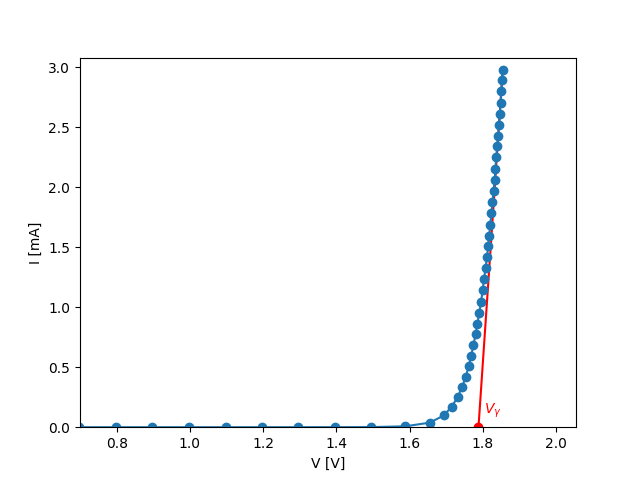
\includegraphics[scale=0.7]{plot diodo LED.png}
    \caption{Plot diodo LED}
    \label{Plot diodo LED}
\end{figure}
\subsubsection{Misura tensione $V_\gamma$ per un diodo Zener}
Lo schema circuitale di quest'esperienza è analogo a quello in figura \ref{fig: Circuito LED} ove al posto del diodo LED è stato posizionato un diodo Zener. Oltre al circuito è equivalente la procedura seguita, tuttavia, a differenza della precedente esperienza, si è data una tensione negativa al generatore per andare a stimare la tensione di Zener. Questa tensione è presente nei diodi Zener in quanto viene innescato l'effetto Zener (da cui ne prende il nome il diodo). Questa tensione non è invece presente nei diodi classici i quali peraltro se polarizzati inversamente potrebbero danneggiarsi (a tensioni molto più alte di quelle di Zener), è pertanto sconsigliato far lavorare diodi classici in quel regime. Il risultato ottenuto è quello riportato in figura \ref{Zener}.\\
Si stima una $V_Z=4.4\unit{\V}$ e una $V_{\gamma}=0.7\unit{\V}$.
\begin{figure}
    \centering
    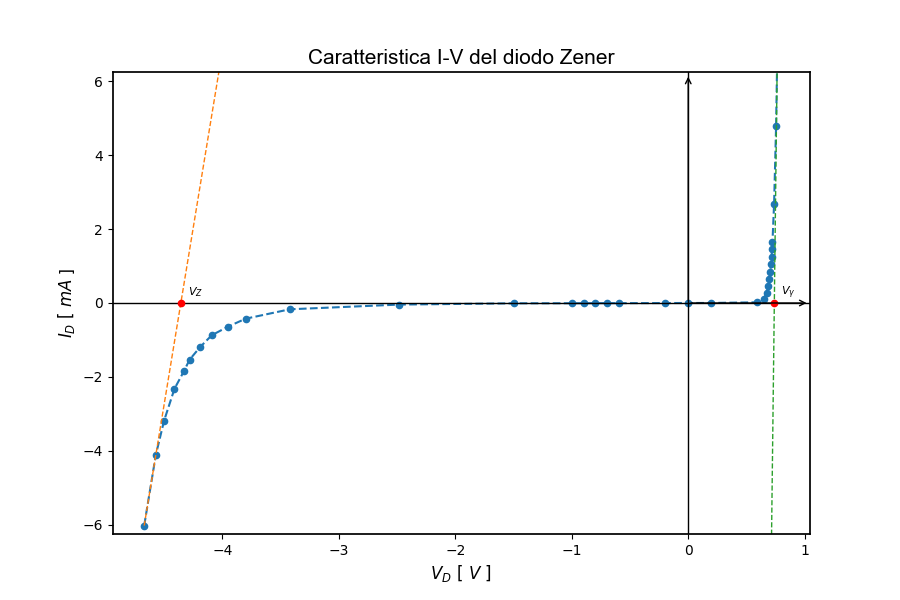
\includegraphics[scale=0.55]{Caratteristica zener.png}
    \caption{Caratteristica I-V di un diodo Zener}
    \label{Zener}
\end{figure}
\subsection{3.2 Diodo come raddrizzatore}
Il diodo è un dispositivo che può essere utilizzato come raddrizzatore d'onda, infatti, per la sua caratteristica di far passare correnti in un verso ma non nell'altro permette, ad esempio, di bloccare potenziali negativi. Lo schema circuitale per vedere questo tipo di fenomeno è quello rappresentato in figura \ref{fig: Raddrizzatore}.
\begin{figure}
    \centering
    \begin{minipage}{0.475\textwidth}
        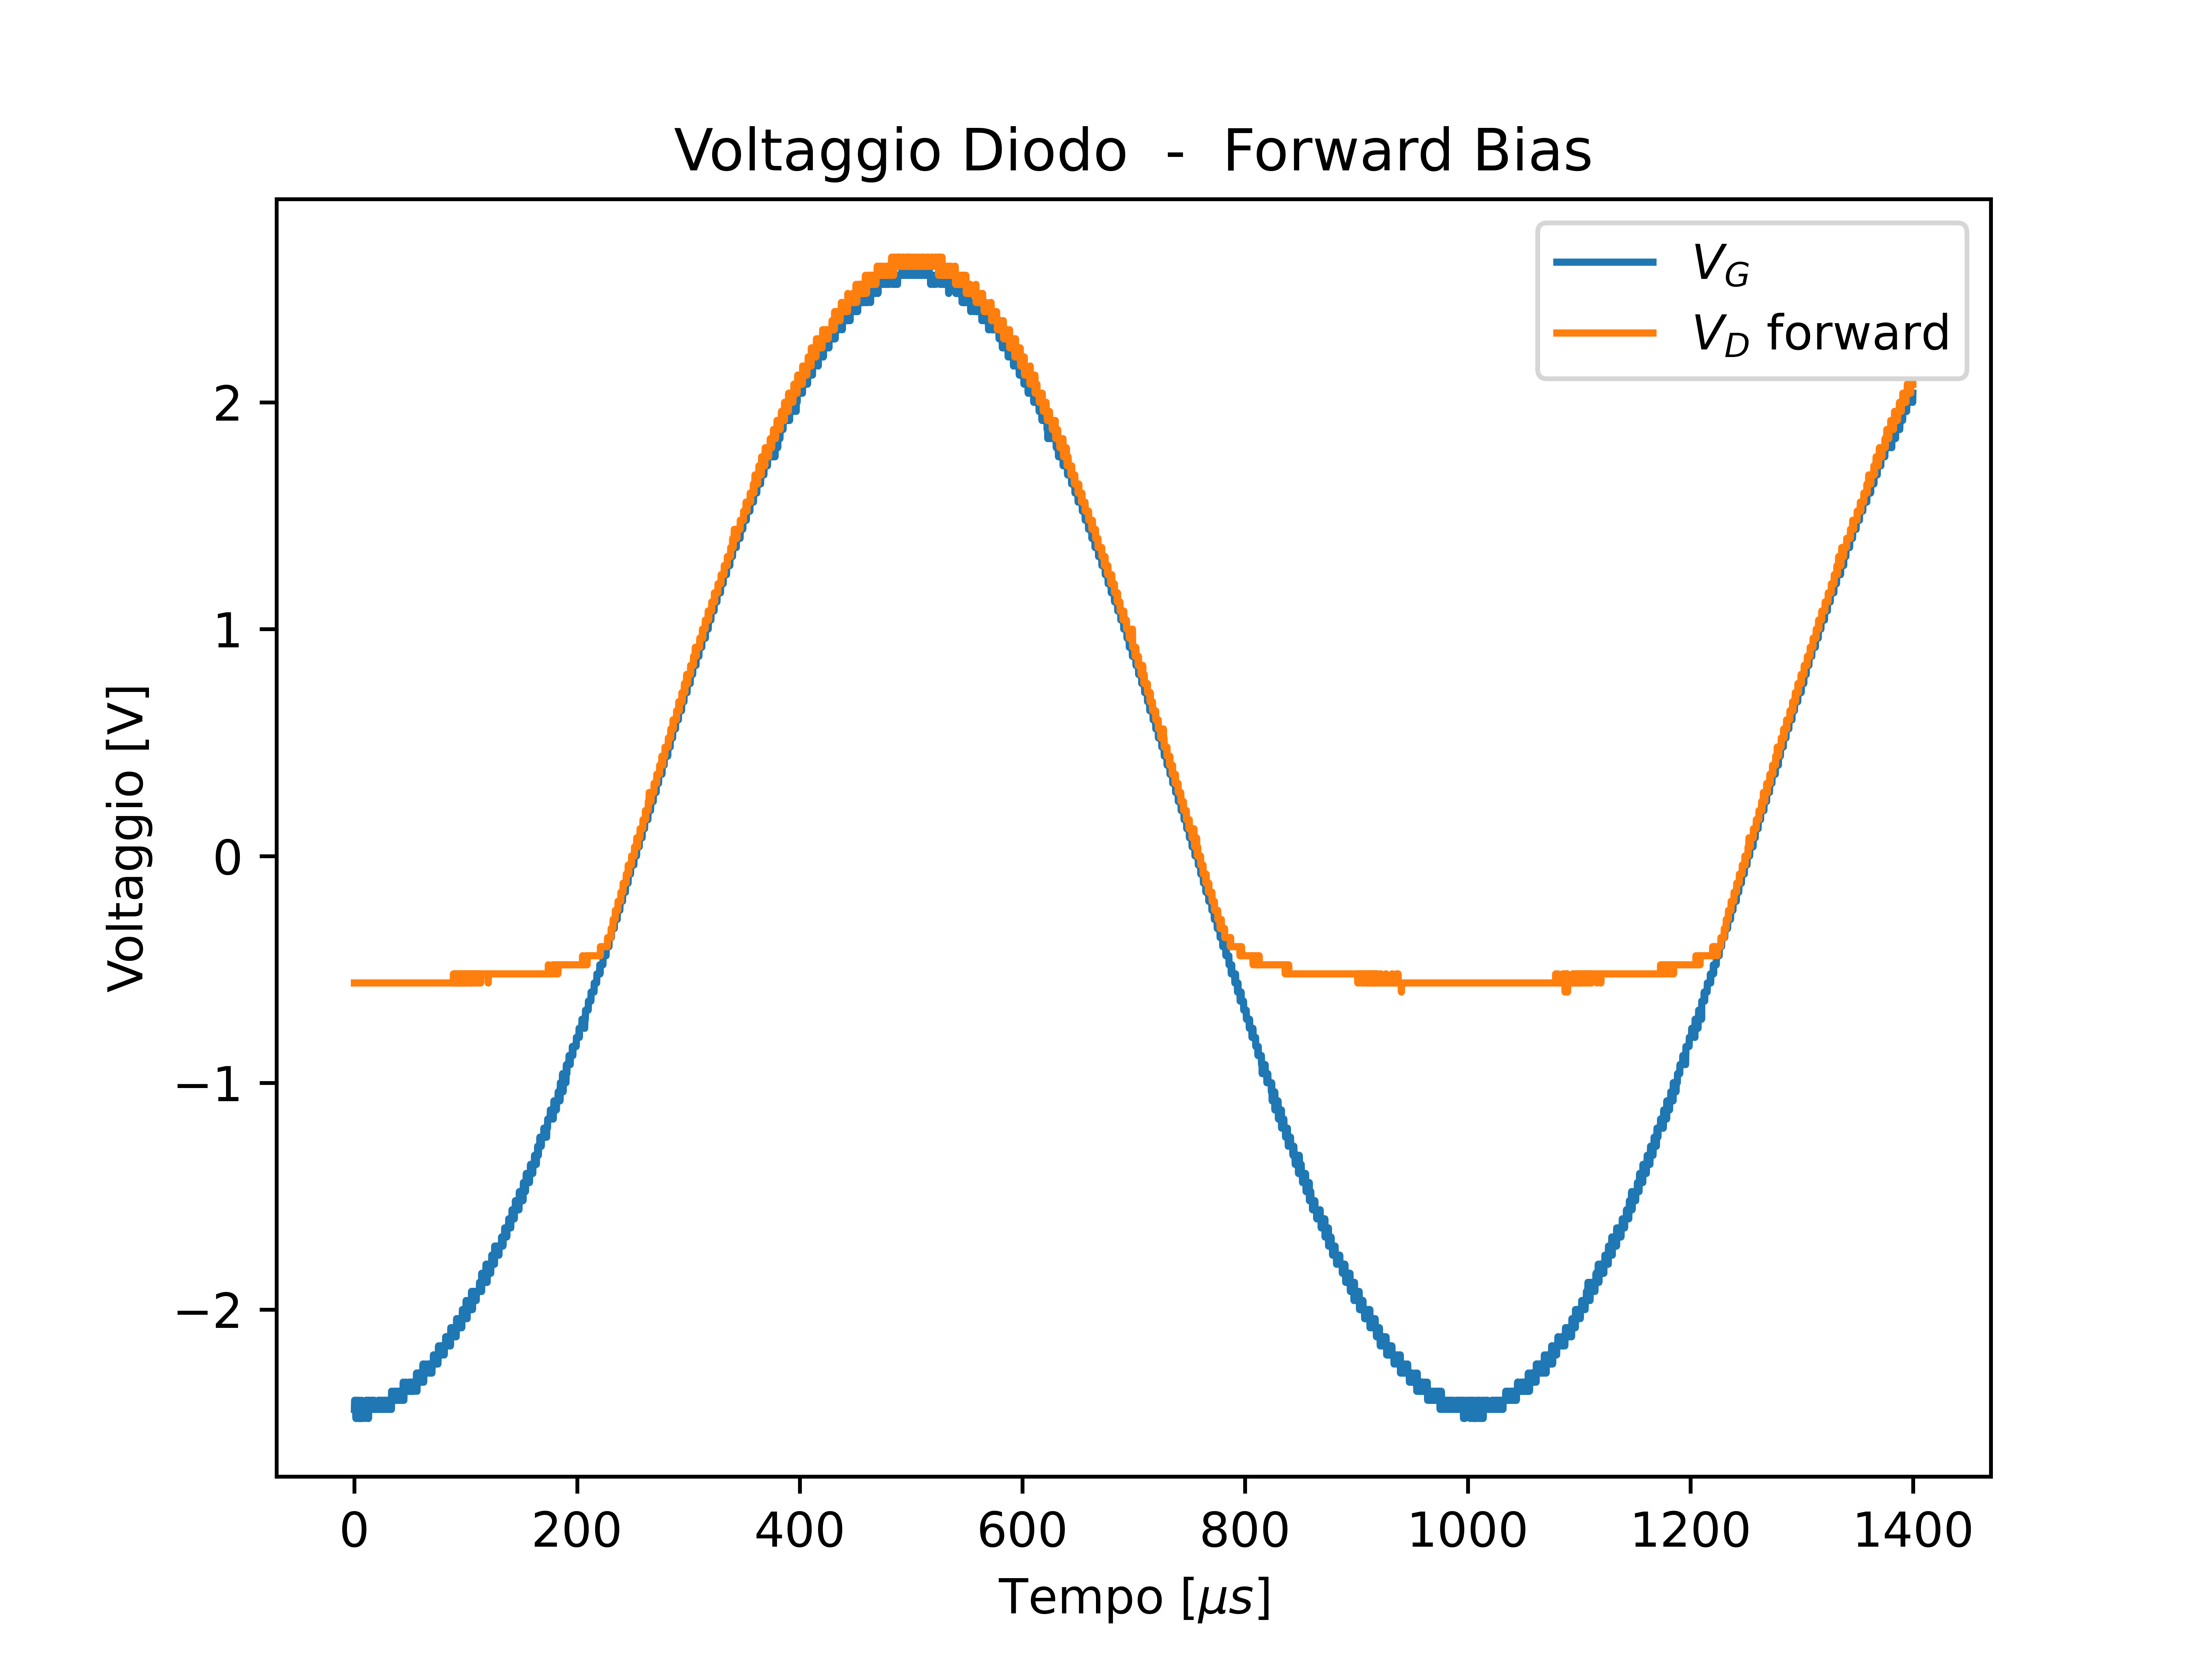
\includegraphics[width=1\textwidth]{Diodo 3.2.(1-2)/V_D_forward.png}
    \label{3.2forwardbias}
    \end{minipage}
    \hfill
    \begin{minipage}{0.475\textwidth}
        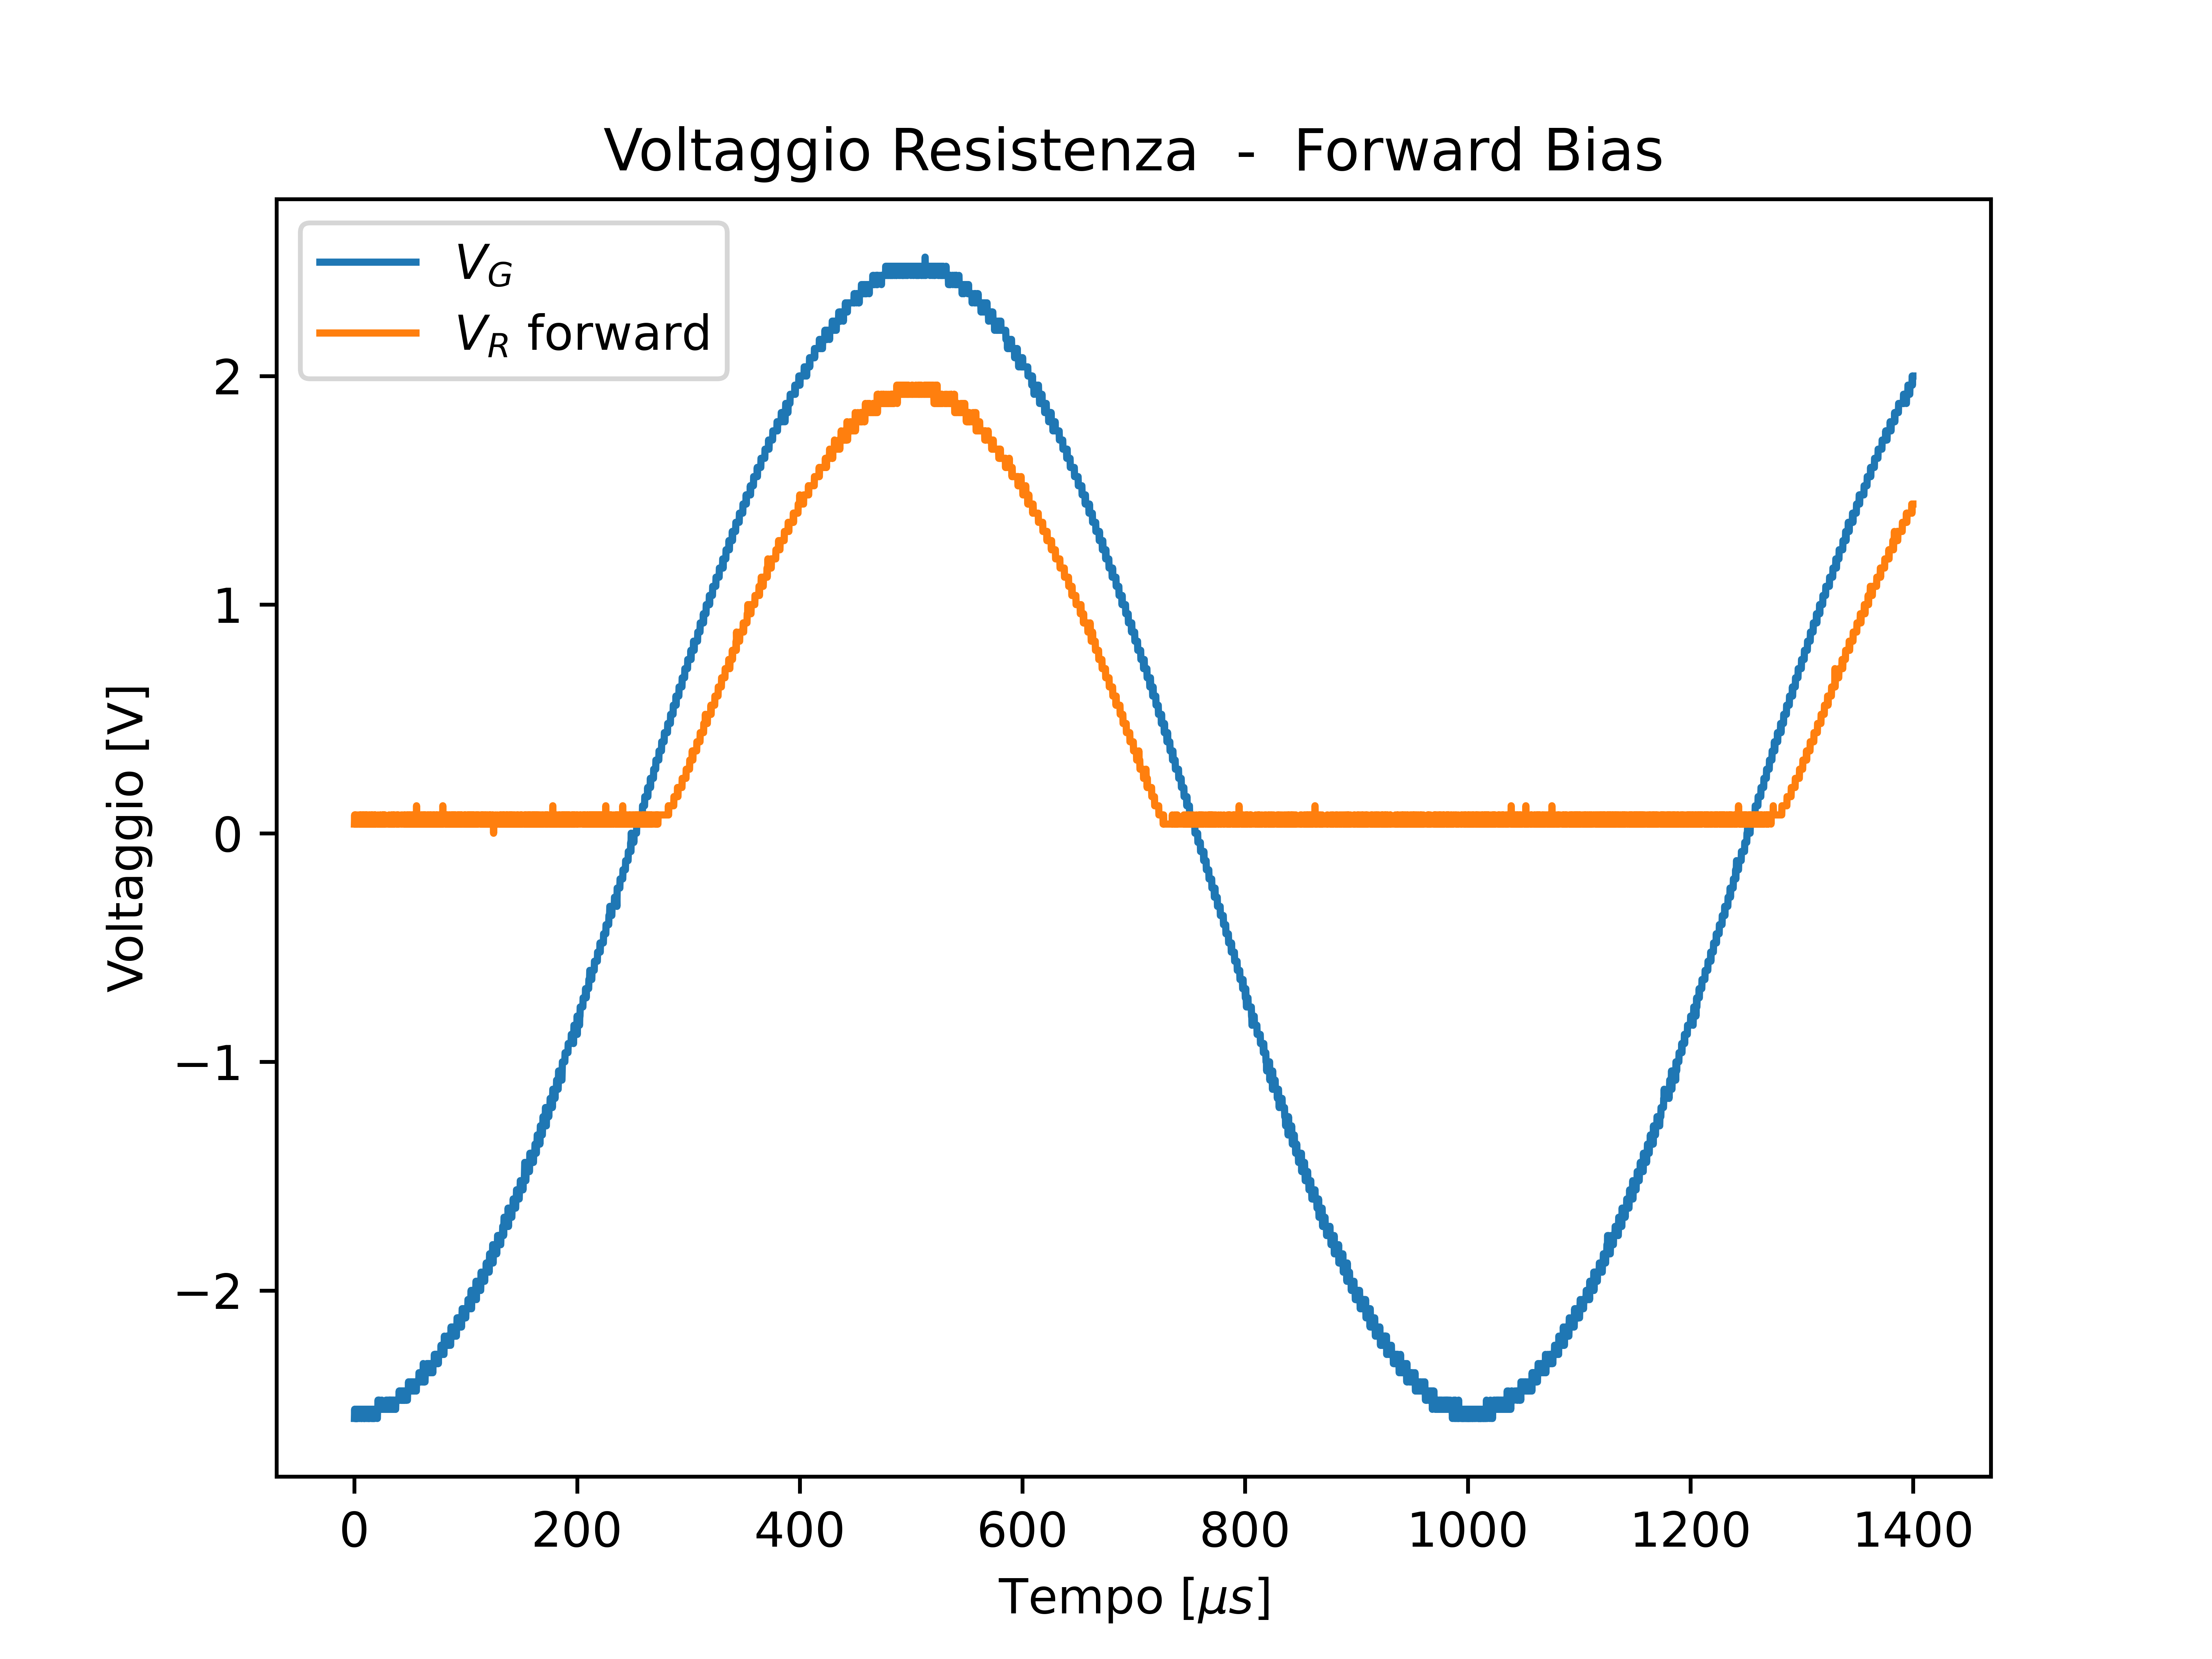
\includegraphics[width=1\textwidth]{Diodo 3.2.(1-2)/V_R_forward.png}
    \end{minipage}
    \caption{Voltaggio ai capi del diodo e della resitenza in forward bias}
    \label{fig:raddrizzatore forward}
\end{figure}
\subsubsection{3.2.1}
Si è utilizzata una resistenza da $1\unit{\kohm}$ e si è data in ingresso una tensione sinusoidale ad una frequenza $f=1\unit{\kHz}$ con tensione $5V_{pp}$.
Si è poi controllato il voltaggio ai capi di R ed ai capi del diodo.
Il risulato è quello rappresentato in figura \ref{fig:raddrizzatore forward}. Come si può notare le tensioni negative sono bloccate dal diodo. Si nota inoltre che la tensione sulla resistenza non raggiunge mai il valore massimo, questa differenza di tensione è proprio la tensione di soglia sul diodo.
\subsubsection{3.2.2}
Si è poi ripetuta la misurazione con il diodo in reversed bias ovvero montato nel verso opposto a come mostrato in figura \ref{fig: Raddrizzatore}. In questo caso il risultato è quello opposto al precedente, vengono pertanto bloccate le tensioni positive come mostra la figura \ref{fig:raddrizzatore reverse}.
\begin{figure}
    \centering
    \begin{minipage}{0.475\textwidth}
        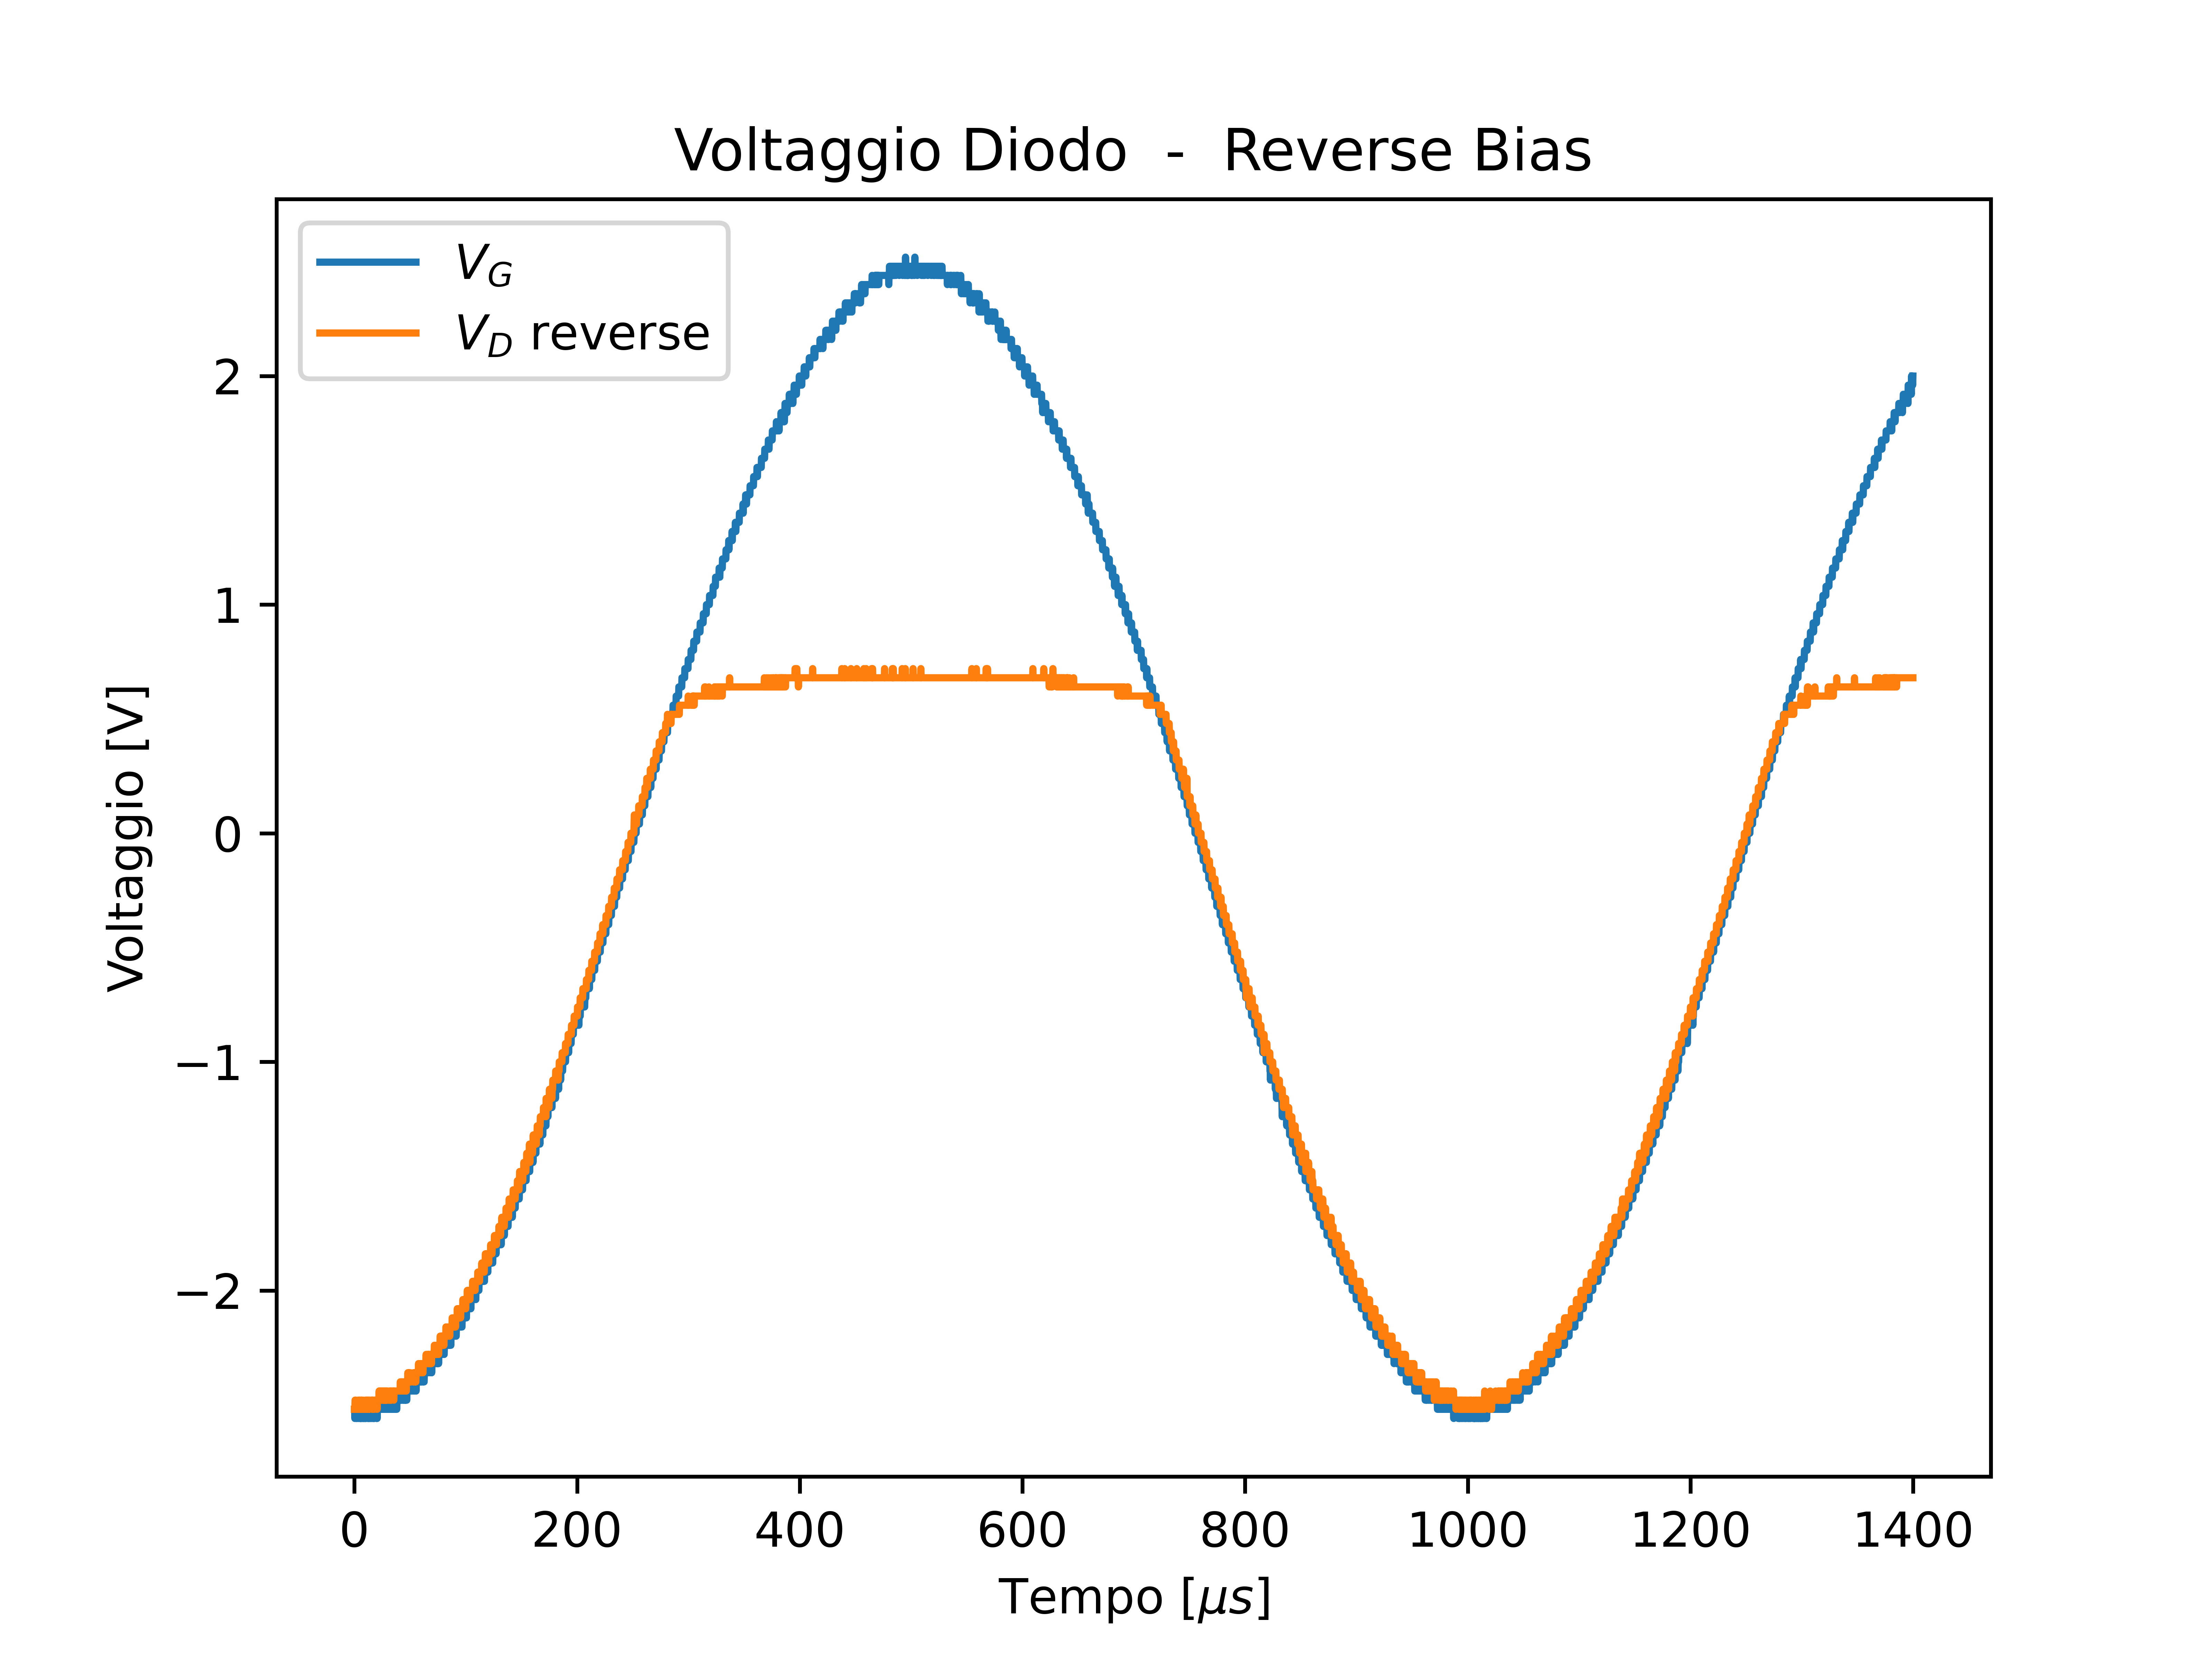
\includegraphics[width=1\textwidth]{Diodo 3.2.(1-2)/V_D_reverse.png}
    \end{minipage}
    \hfill
    \begin{minipage}{0.475\textwidth}
        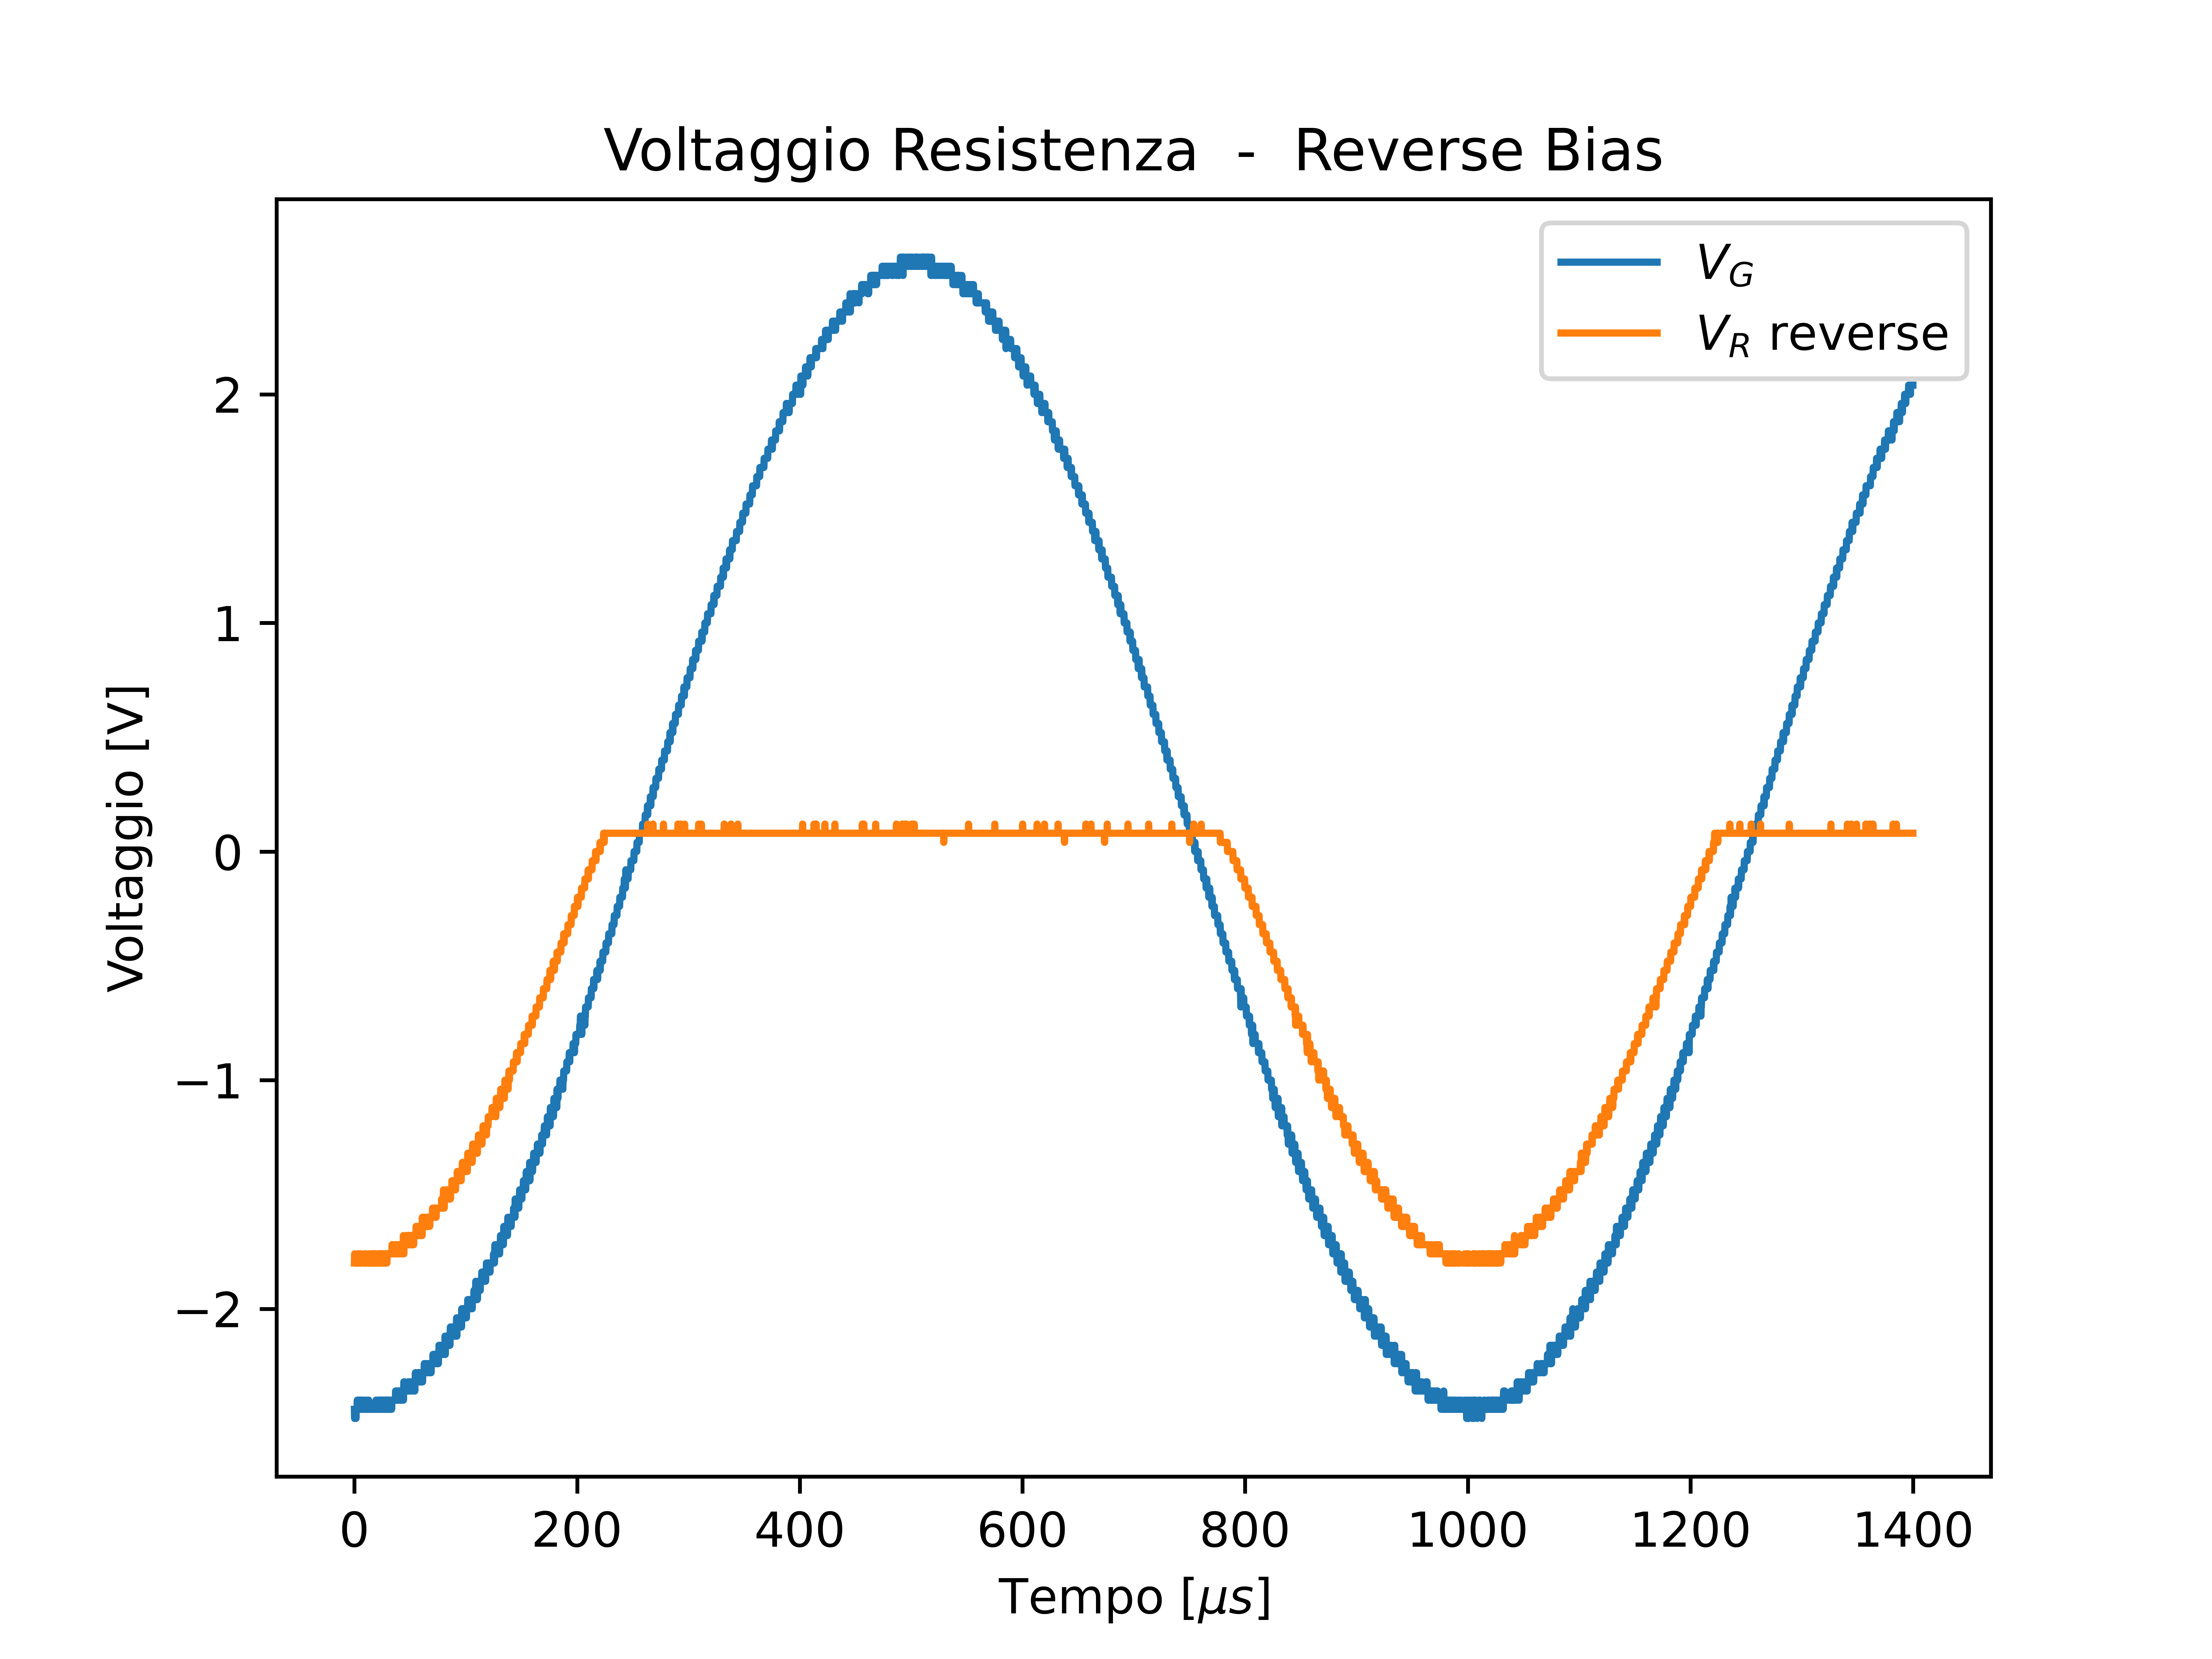
\includegraphics[width=1\textwidth]{Diodo 3.2.(1-2)/V_R_reverse.png}
    \end{minipage}
    \caption{Voltaggio ai capi del diodo e della resitenza in forward bias}
    \label{fig:raddrizzatore reverse}
\end{figure}
\subsubsection{3.2.3}
Misure analoghe sono state svolte anche per tensioni di ingresso ad onda triangolare. Il risultato di tali misure è riportato in figura \ref{Triangular input}.\\
Il risulato è pressocchè analogo.
\begin{figure}
    \centering
    \begin{minipage}{0.475\textwidth}
        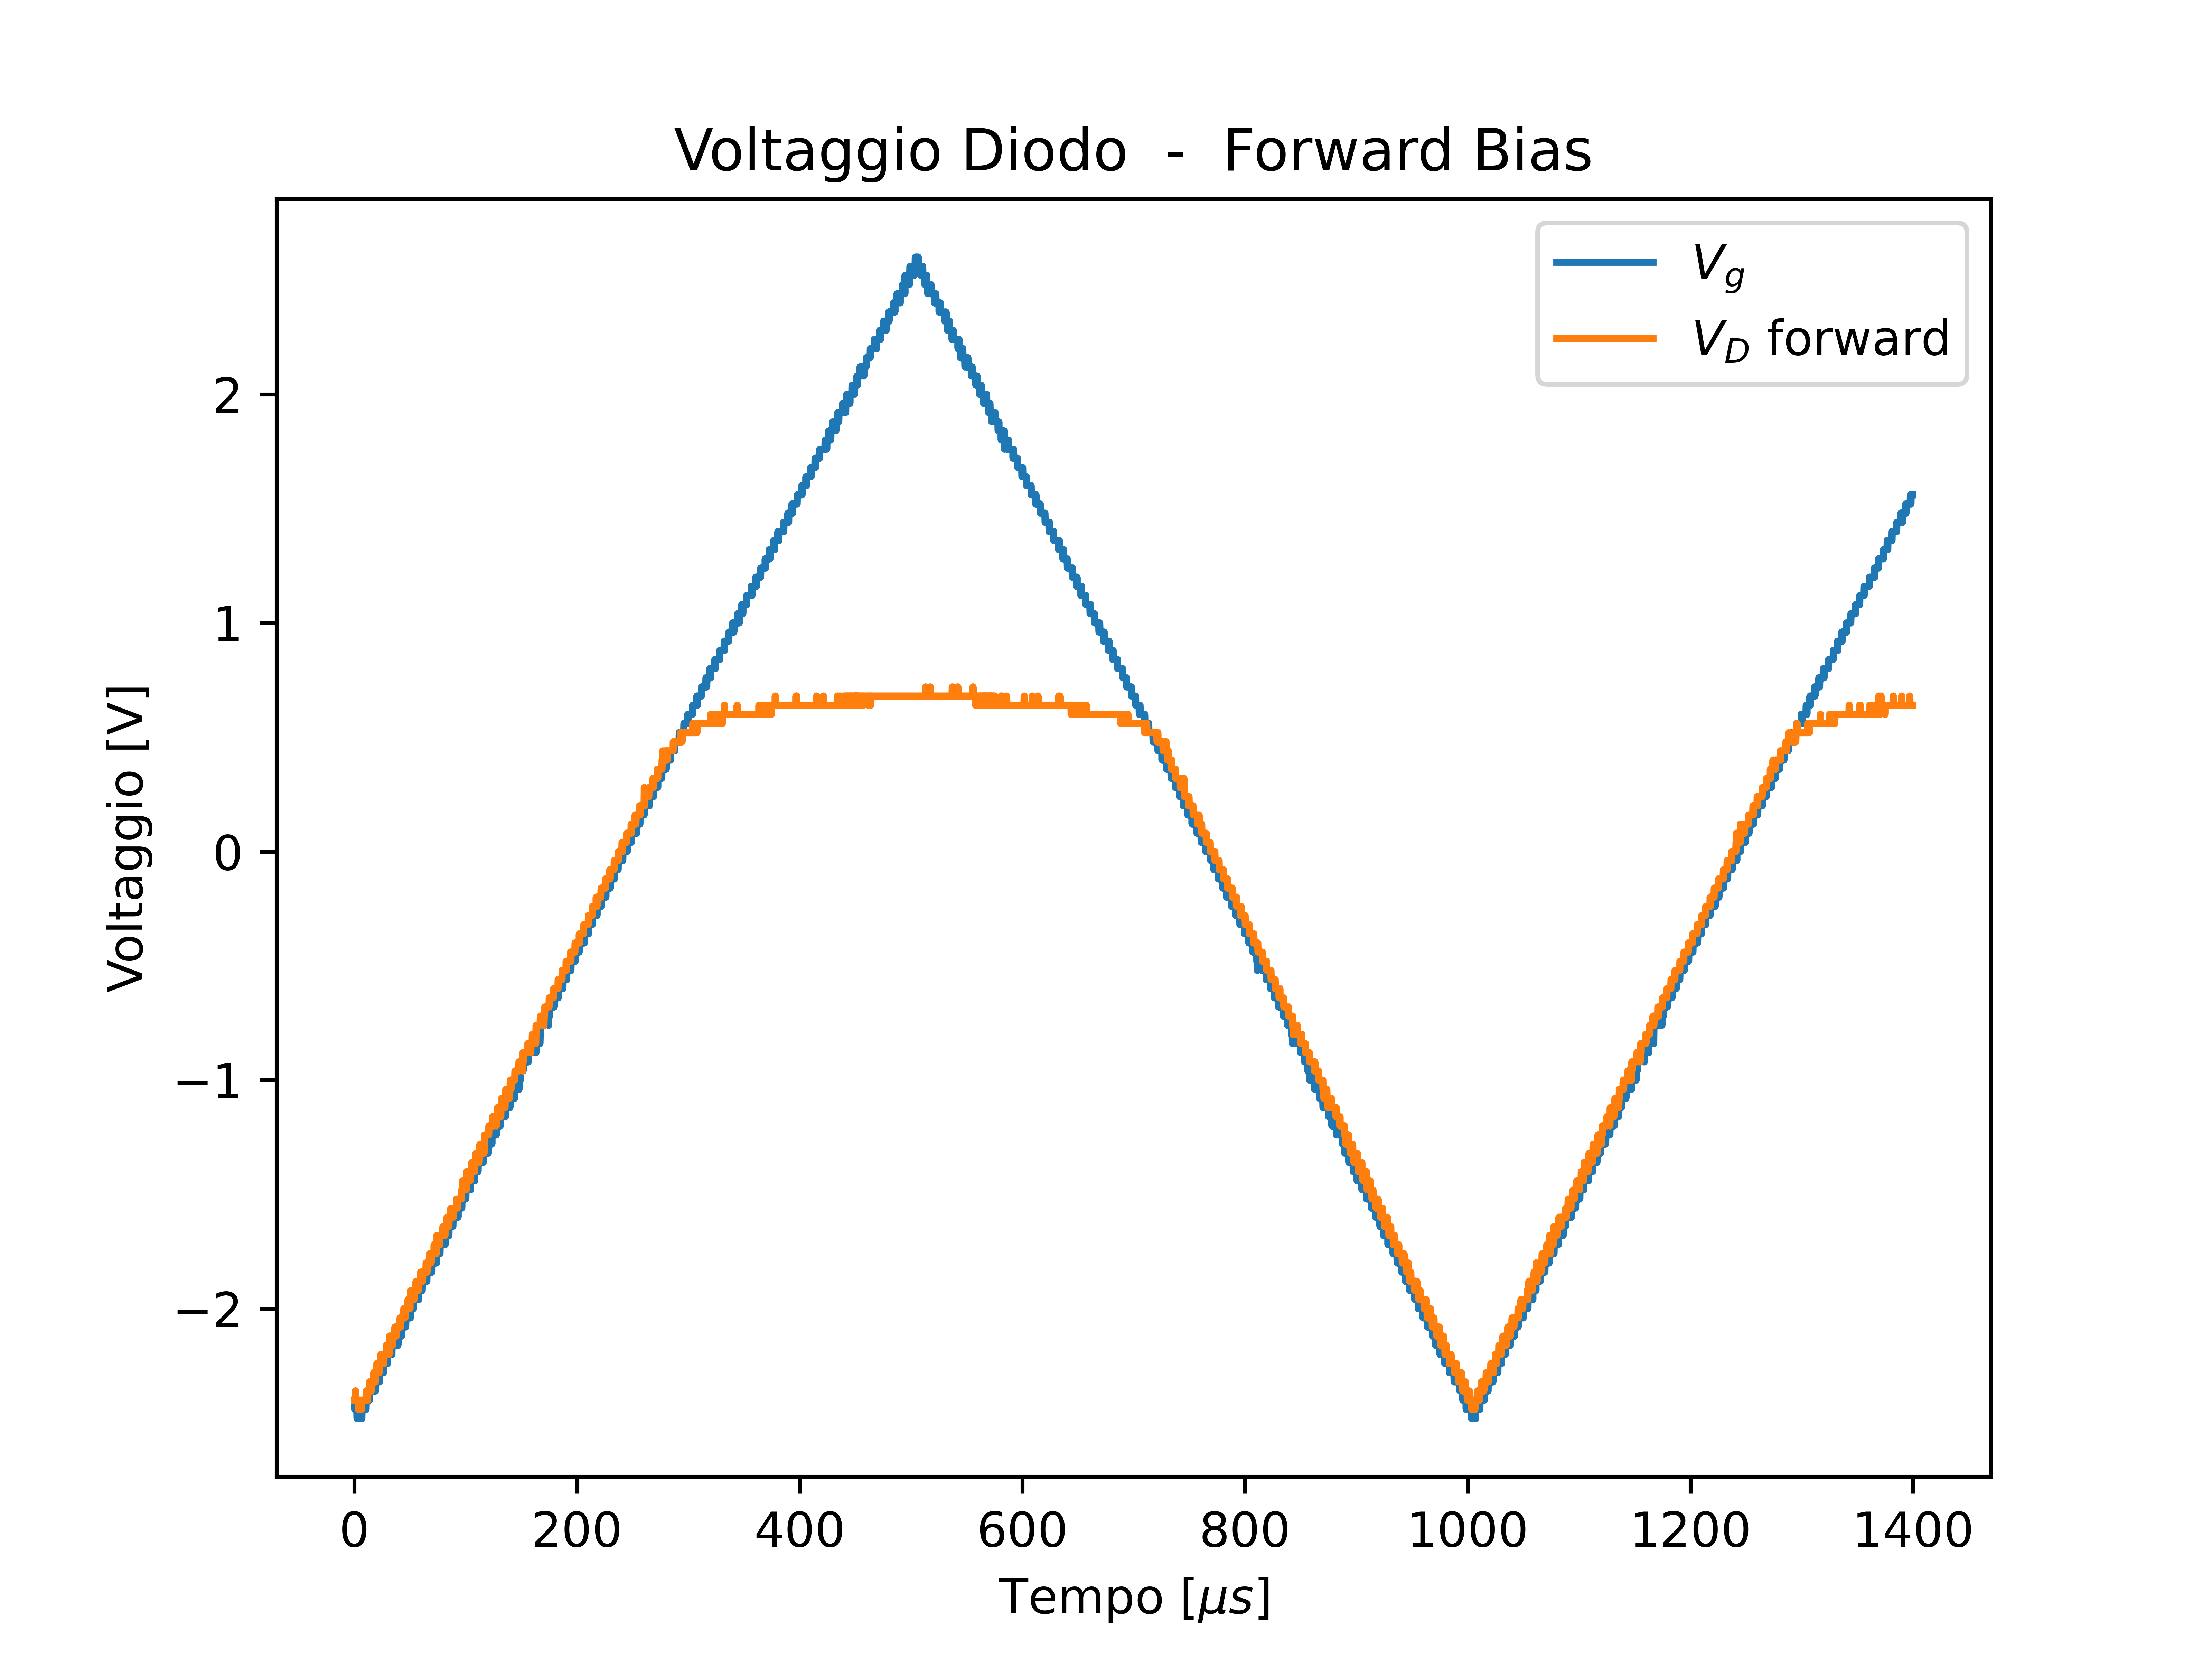
\includegraphics[width=1\textwidth]{Diodo 3.2.3/Triang_V_D_Forward.png}
    \end{minipage}
    \hfill
    \begin{minipage}{0.475\textwidth}
        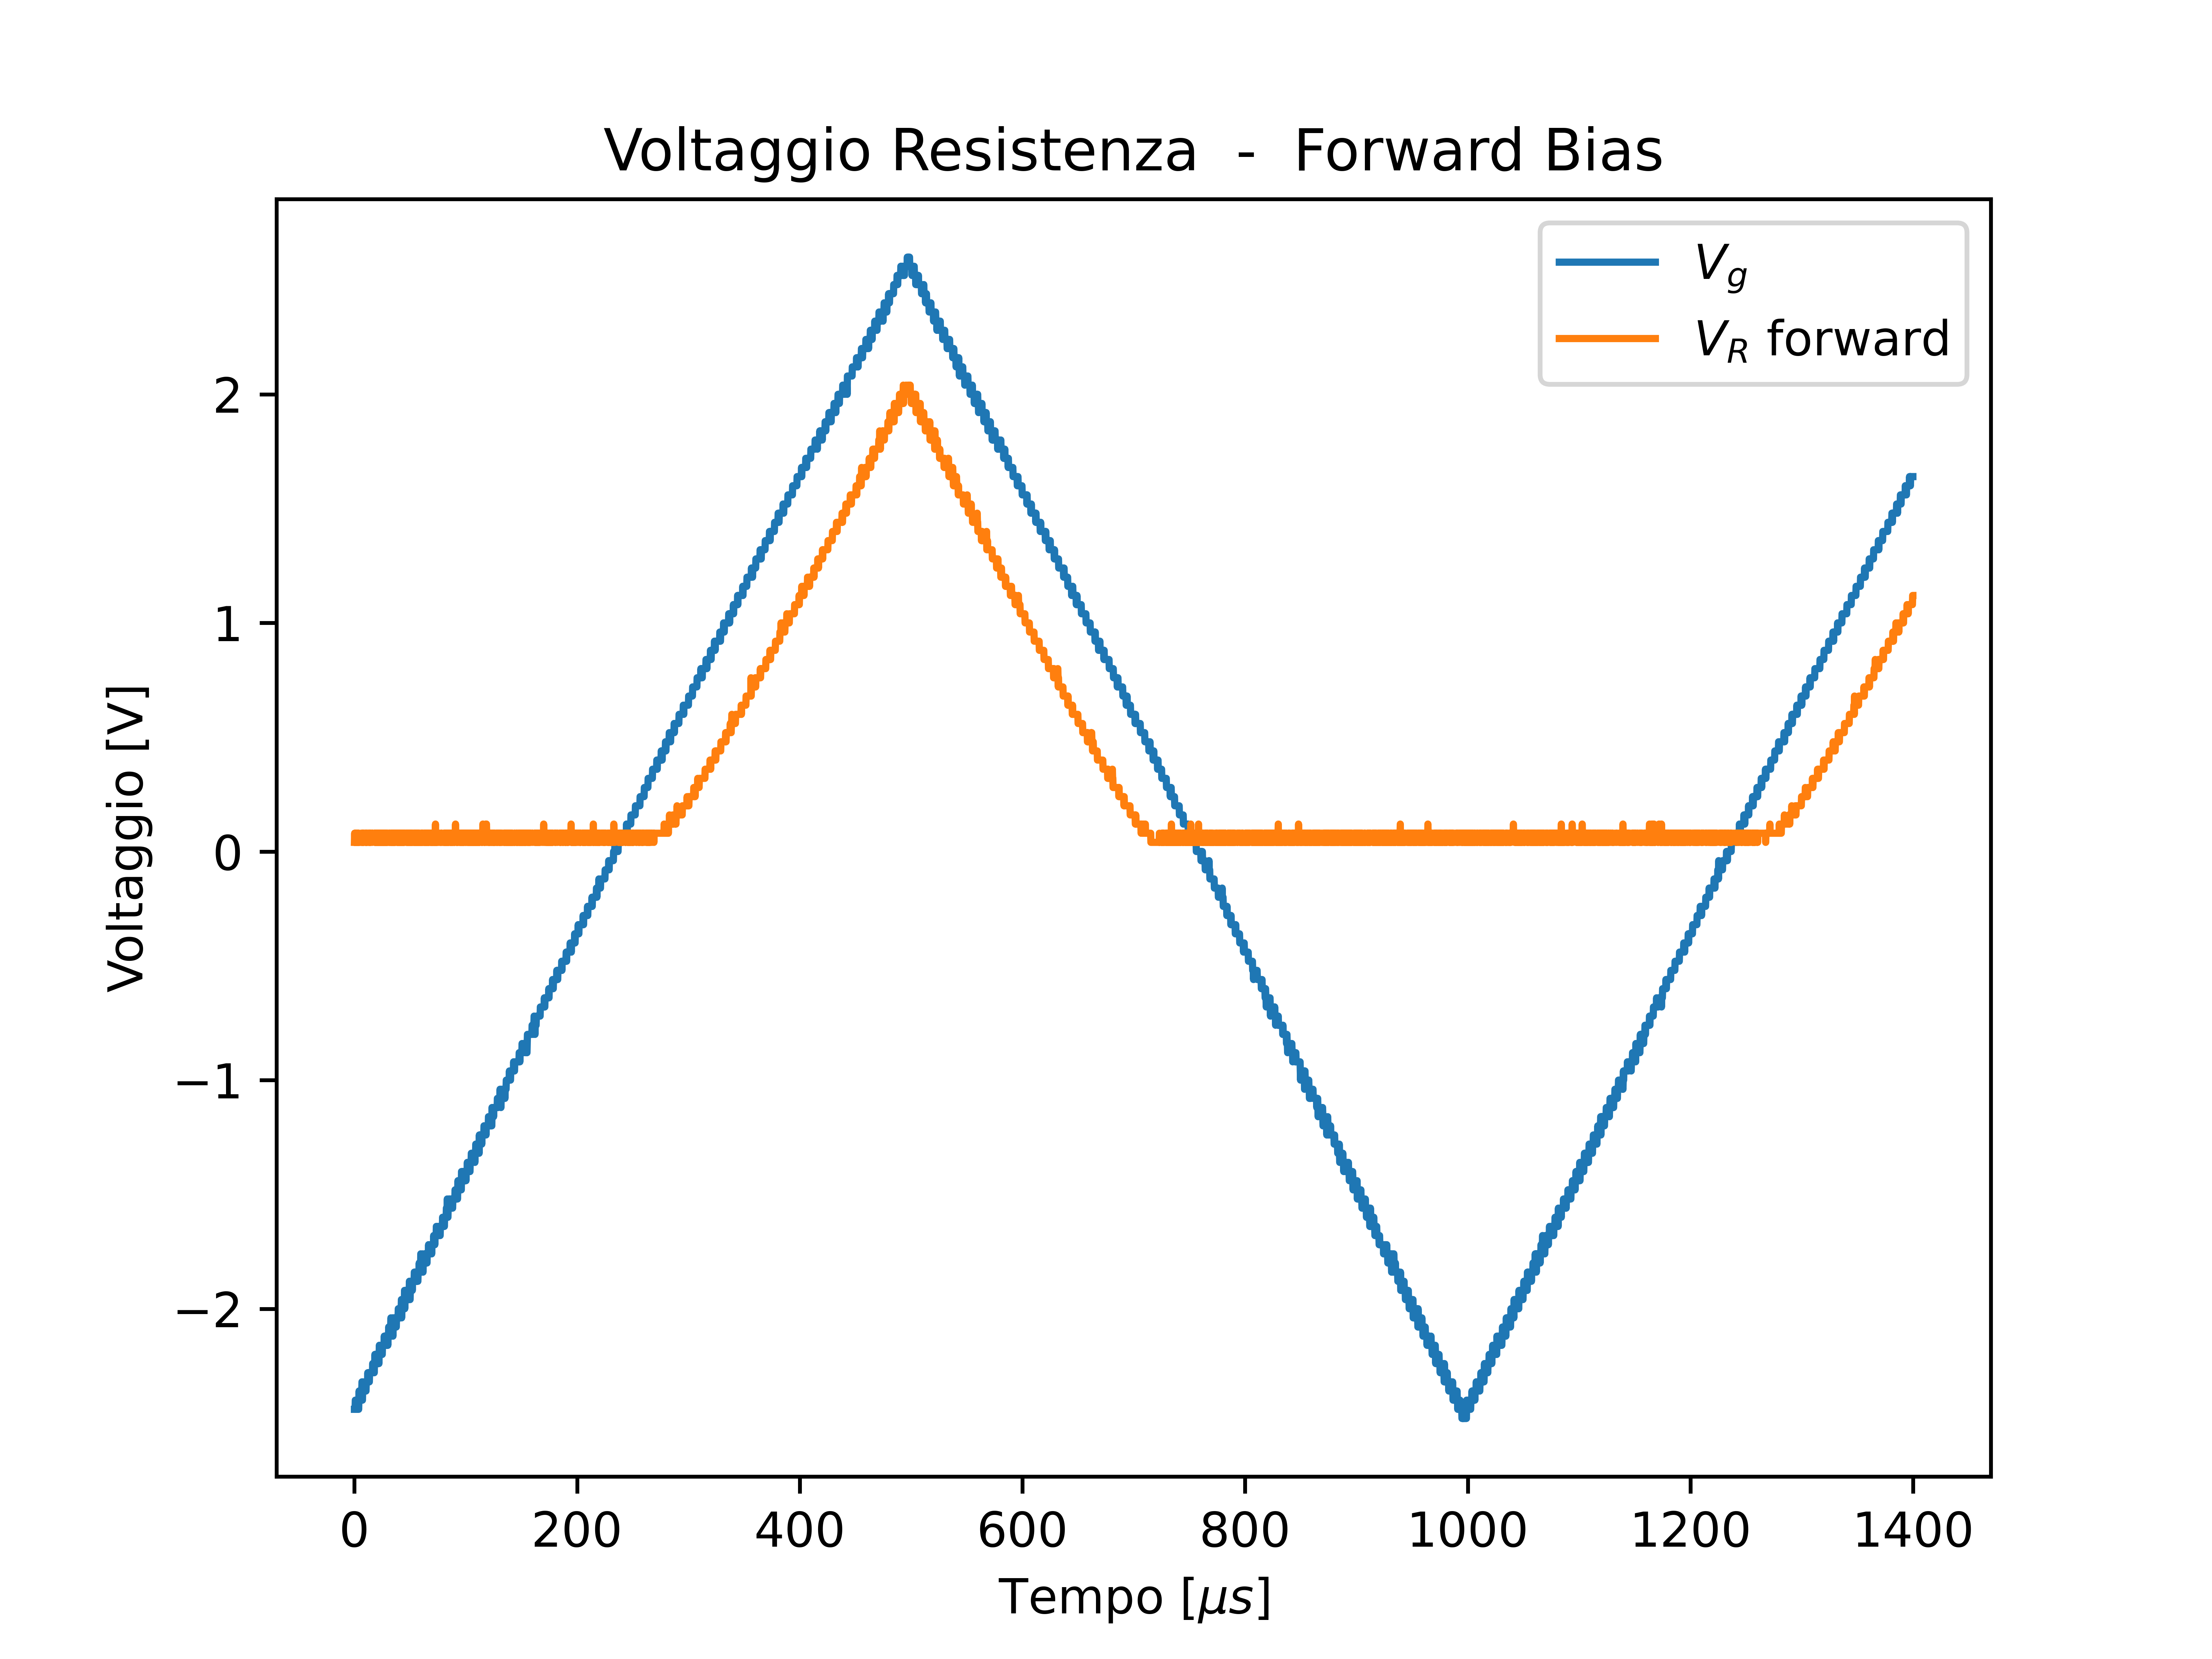
\includegraphics[width=1\textwidth]{Diodo 3.2.3/Triang_V_R_Forward.png}
    \end{minipage}
    \begin{minipage}{0.475\textwidth}
        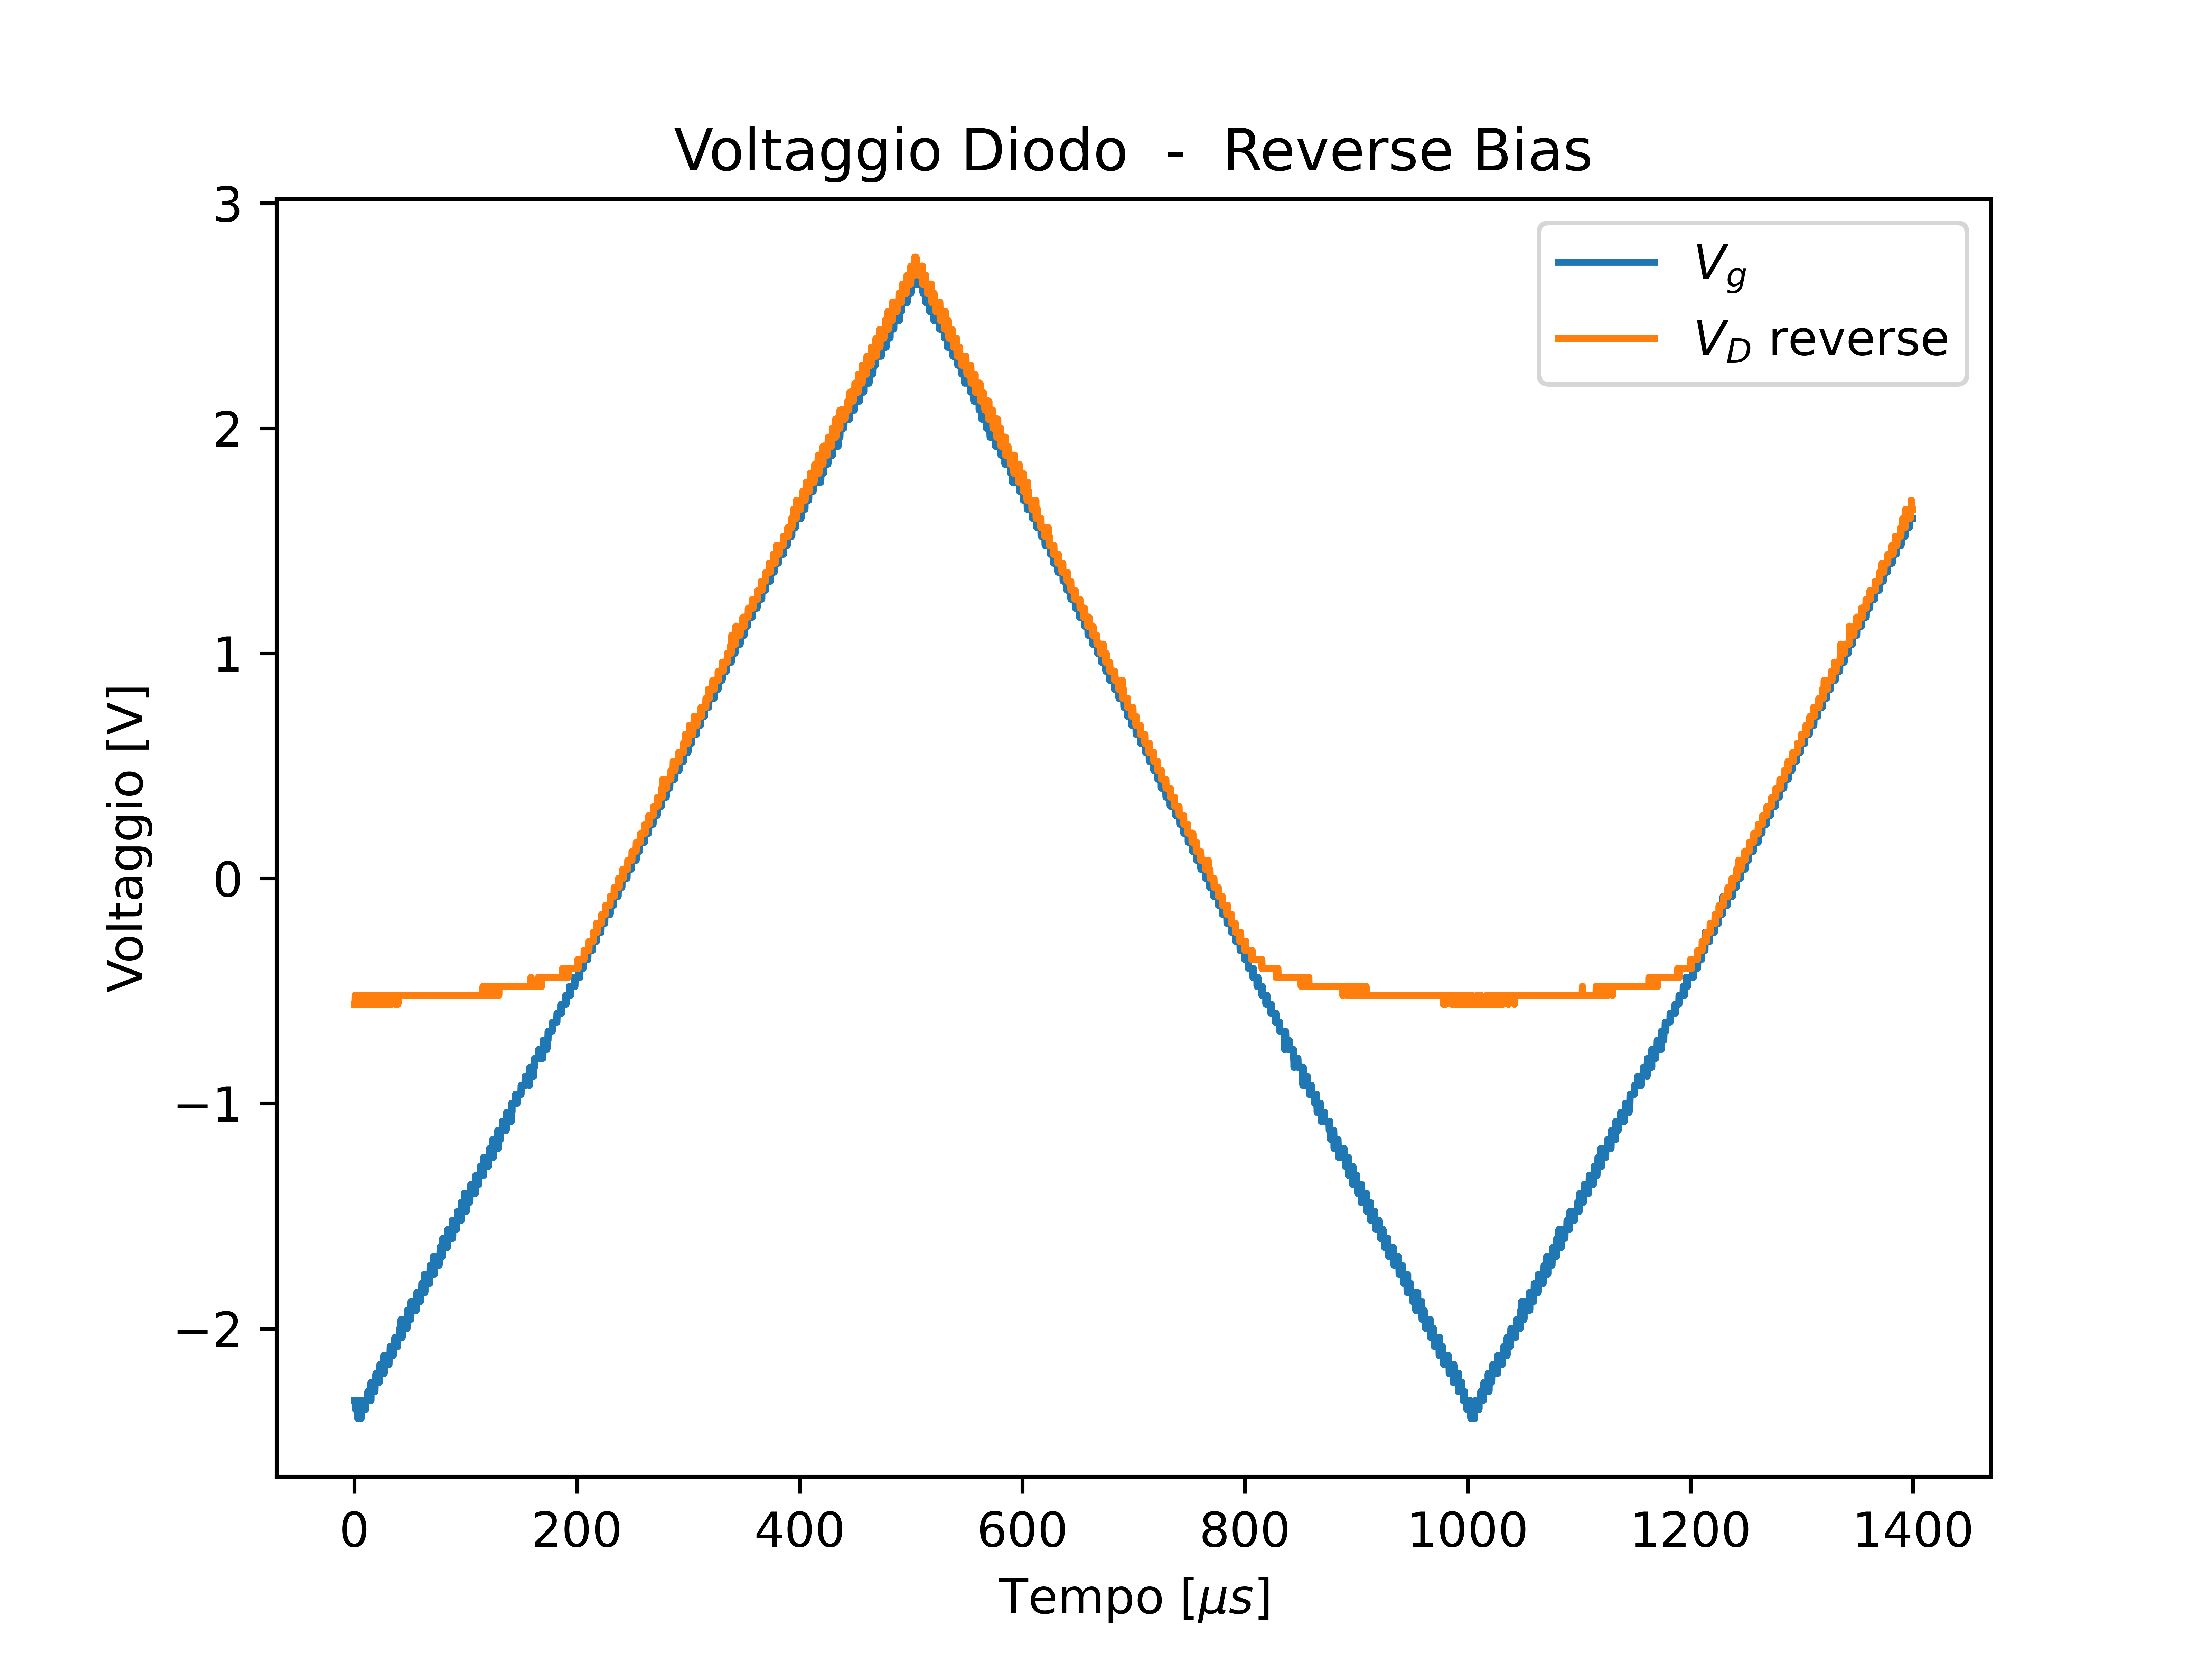
\includegraphics[width=1\textwidth]{Diodo 3.2.3/Triang_V_D_Reverse.png}
    \end{minipage}
    \hfill
    \begin{minipage}{0.475\textwidth}
        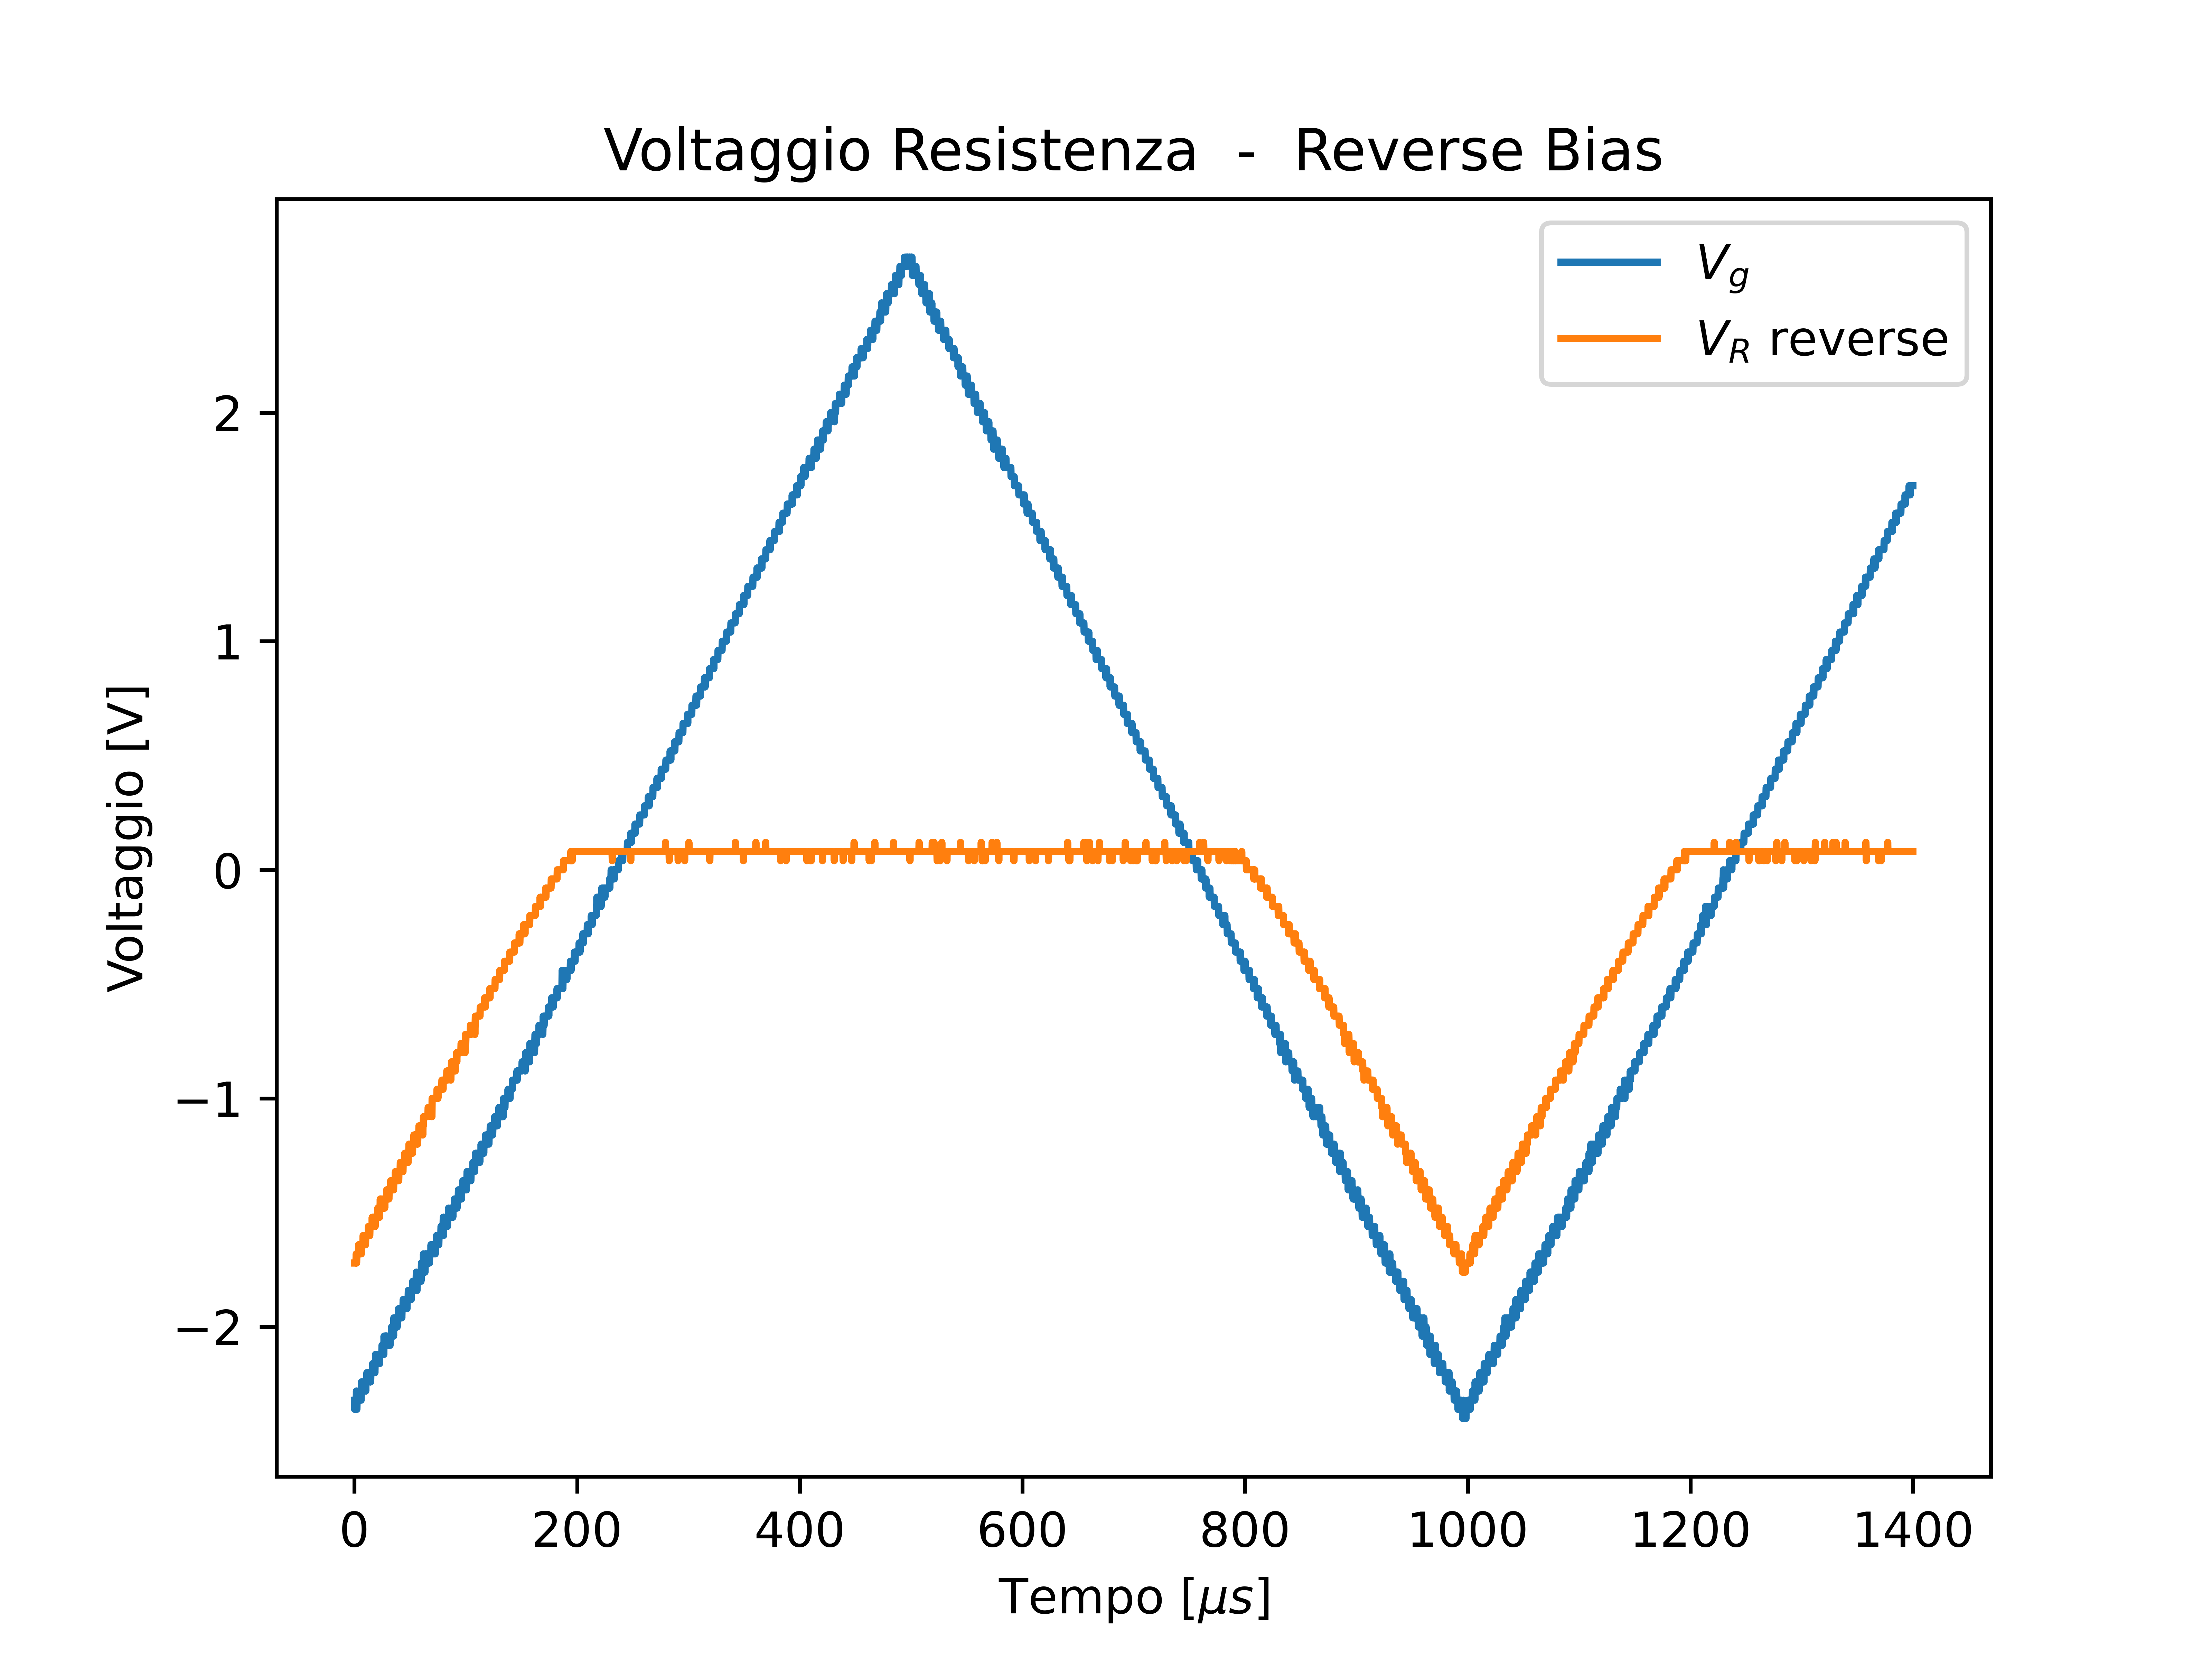
\includegraphics[width=1\textwidth]{Diodo 3.2.3/Triang_V_R_Reverse.png}
    \end{minipage}
    \caption{Voltaggio ai capi di diodo e resistenza con voltaggio in ingresso pari ad un'onda triangolare }
    \label{Triangular input}
\end{figure}
\subsubsection{3.2.4}
In quest'attività si è studiato il comportamento del circuito mostrato in figura \ref{fig: Raddrizzatore} a destra.
La differenza quindi con il circuito precedente è la presenza di un generatore di tensione costante a valle del diodo.\\
L'aggiunta di questo generatore di tensione ha portato delle complicazioni sulla misurazione effettiva in laboratorio della tensione ai capi del diodo in quanto sia il generatore di tensione che l'oscilloscopio richiedono il collegamento a massa.\\
Il risultato di tale misura è quello riportato in figura \ref{3.2.4}.
\subsubsection{3.2.5}
Esattamente come per il circuito precedente si è invertita la polarità del diodo e sono state riprese le misure e si sono quindi ottenuti i risultati in figura \ref{}
\begin{figure}
    \begin{minipage}{0.475\textwidth}
        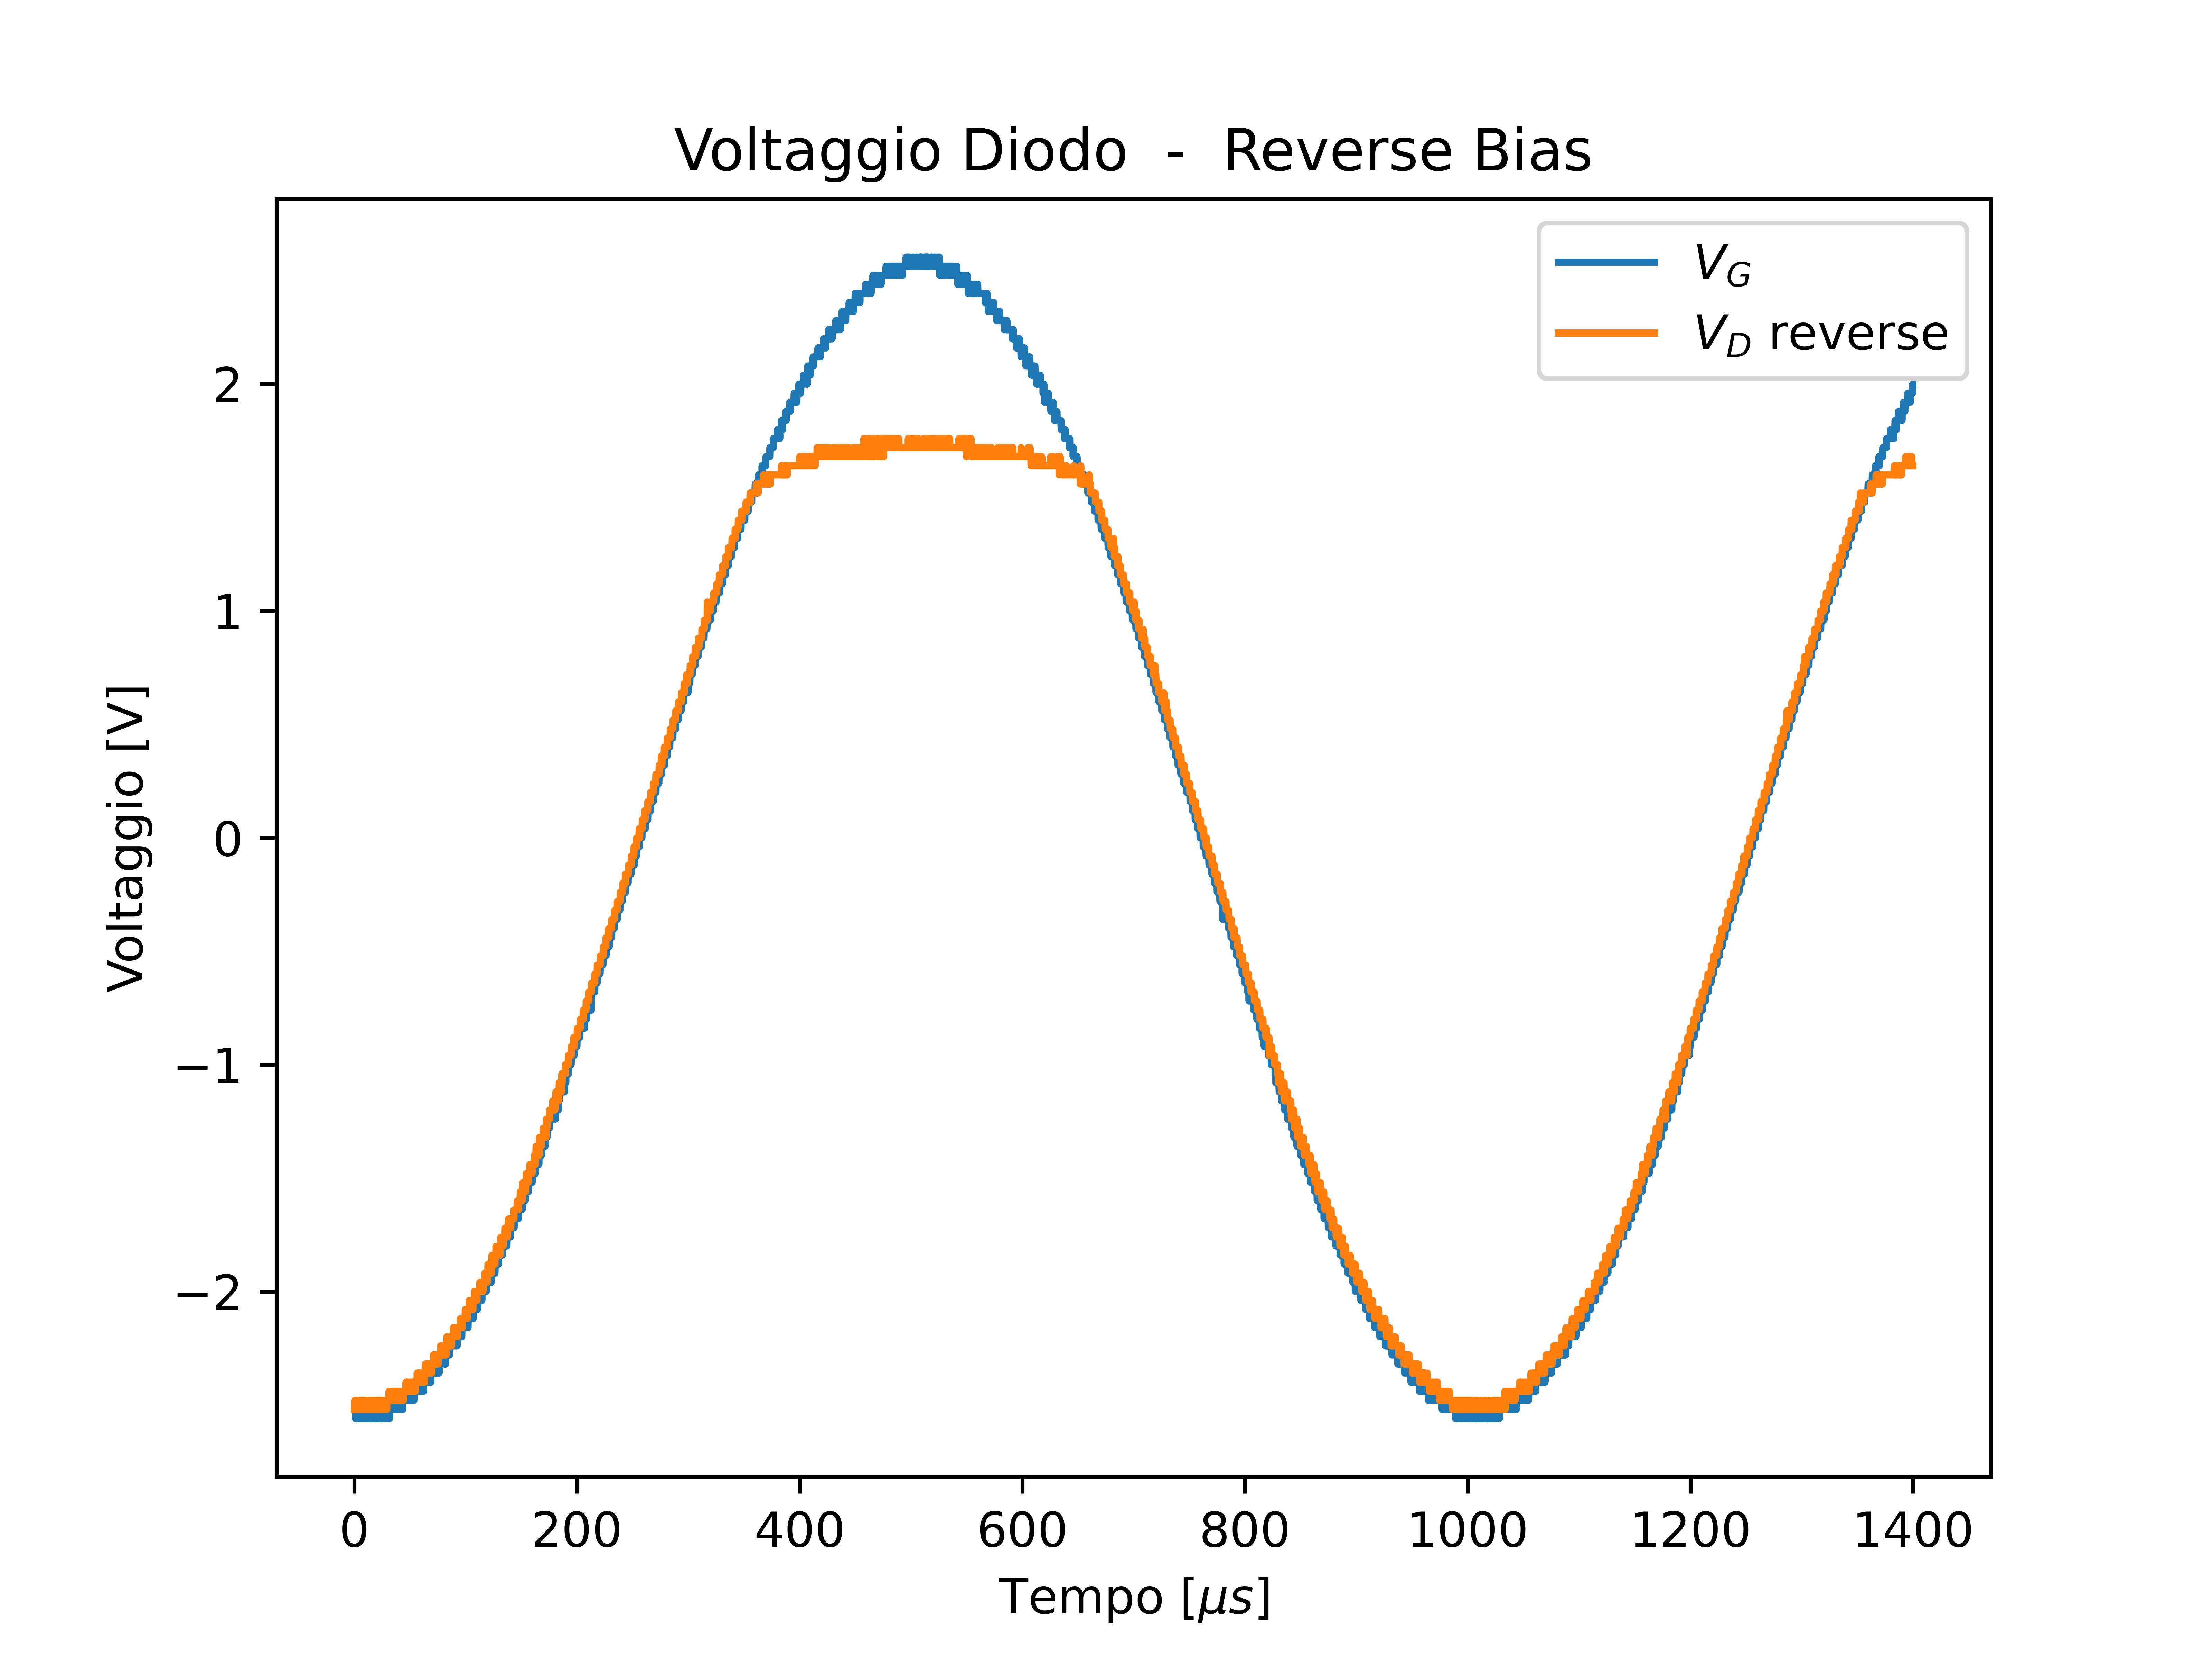
\includegraphics[width=1\textwidth]{Diodo 3.2.(4-5)/DC_V_D_Reverse.png}
    \end{minipage}
    \hfill
    \begin{minipage}{0.475\textwidth}
        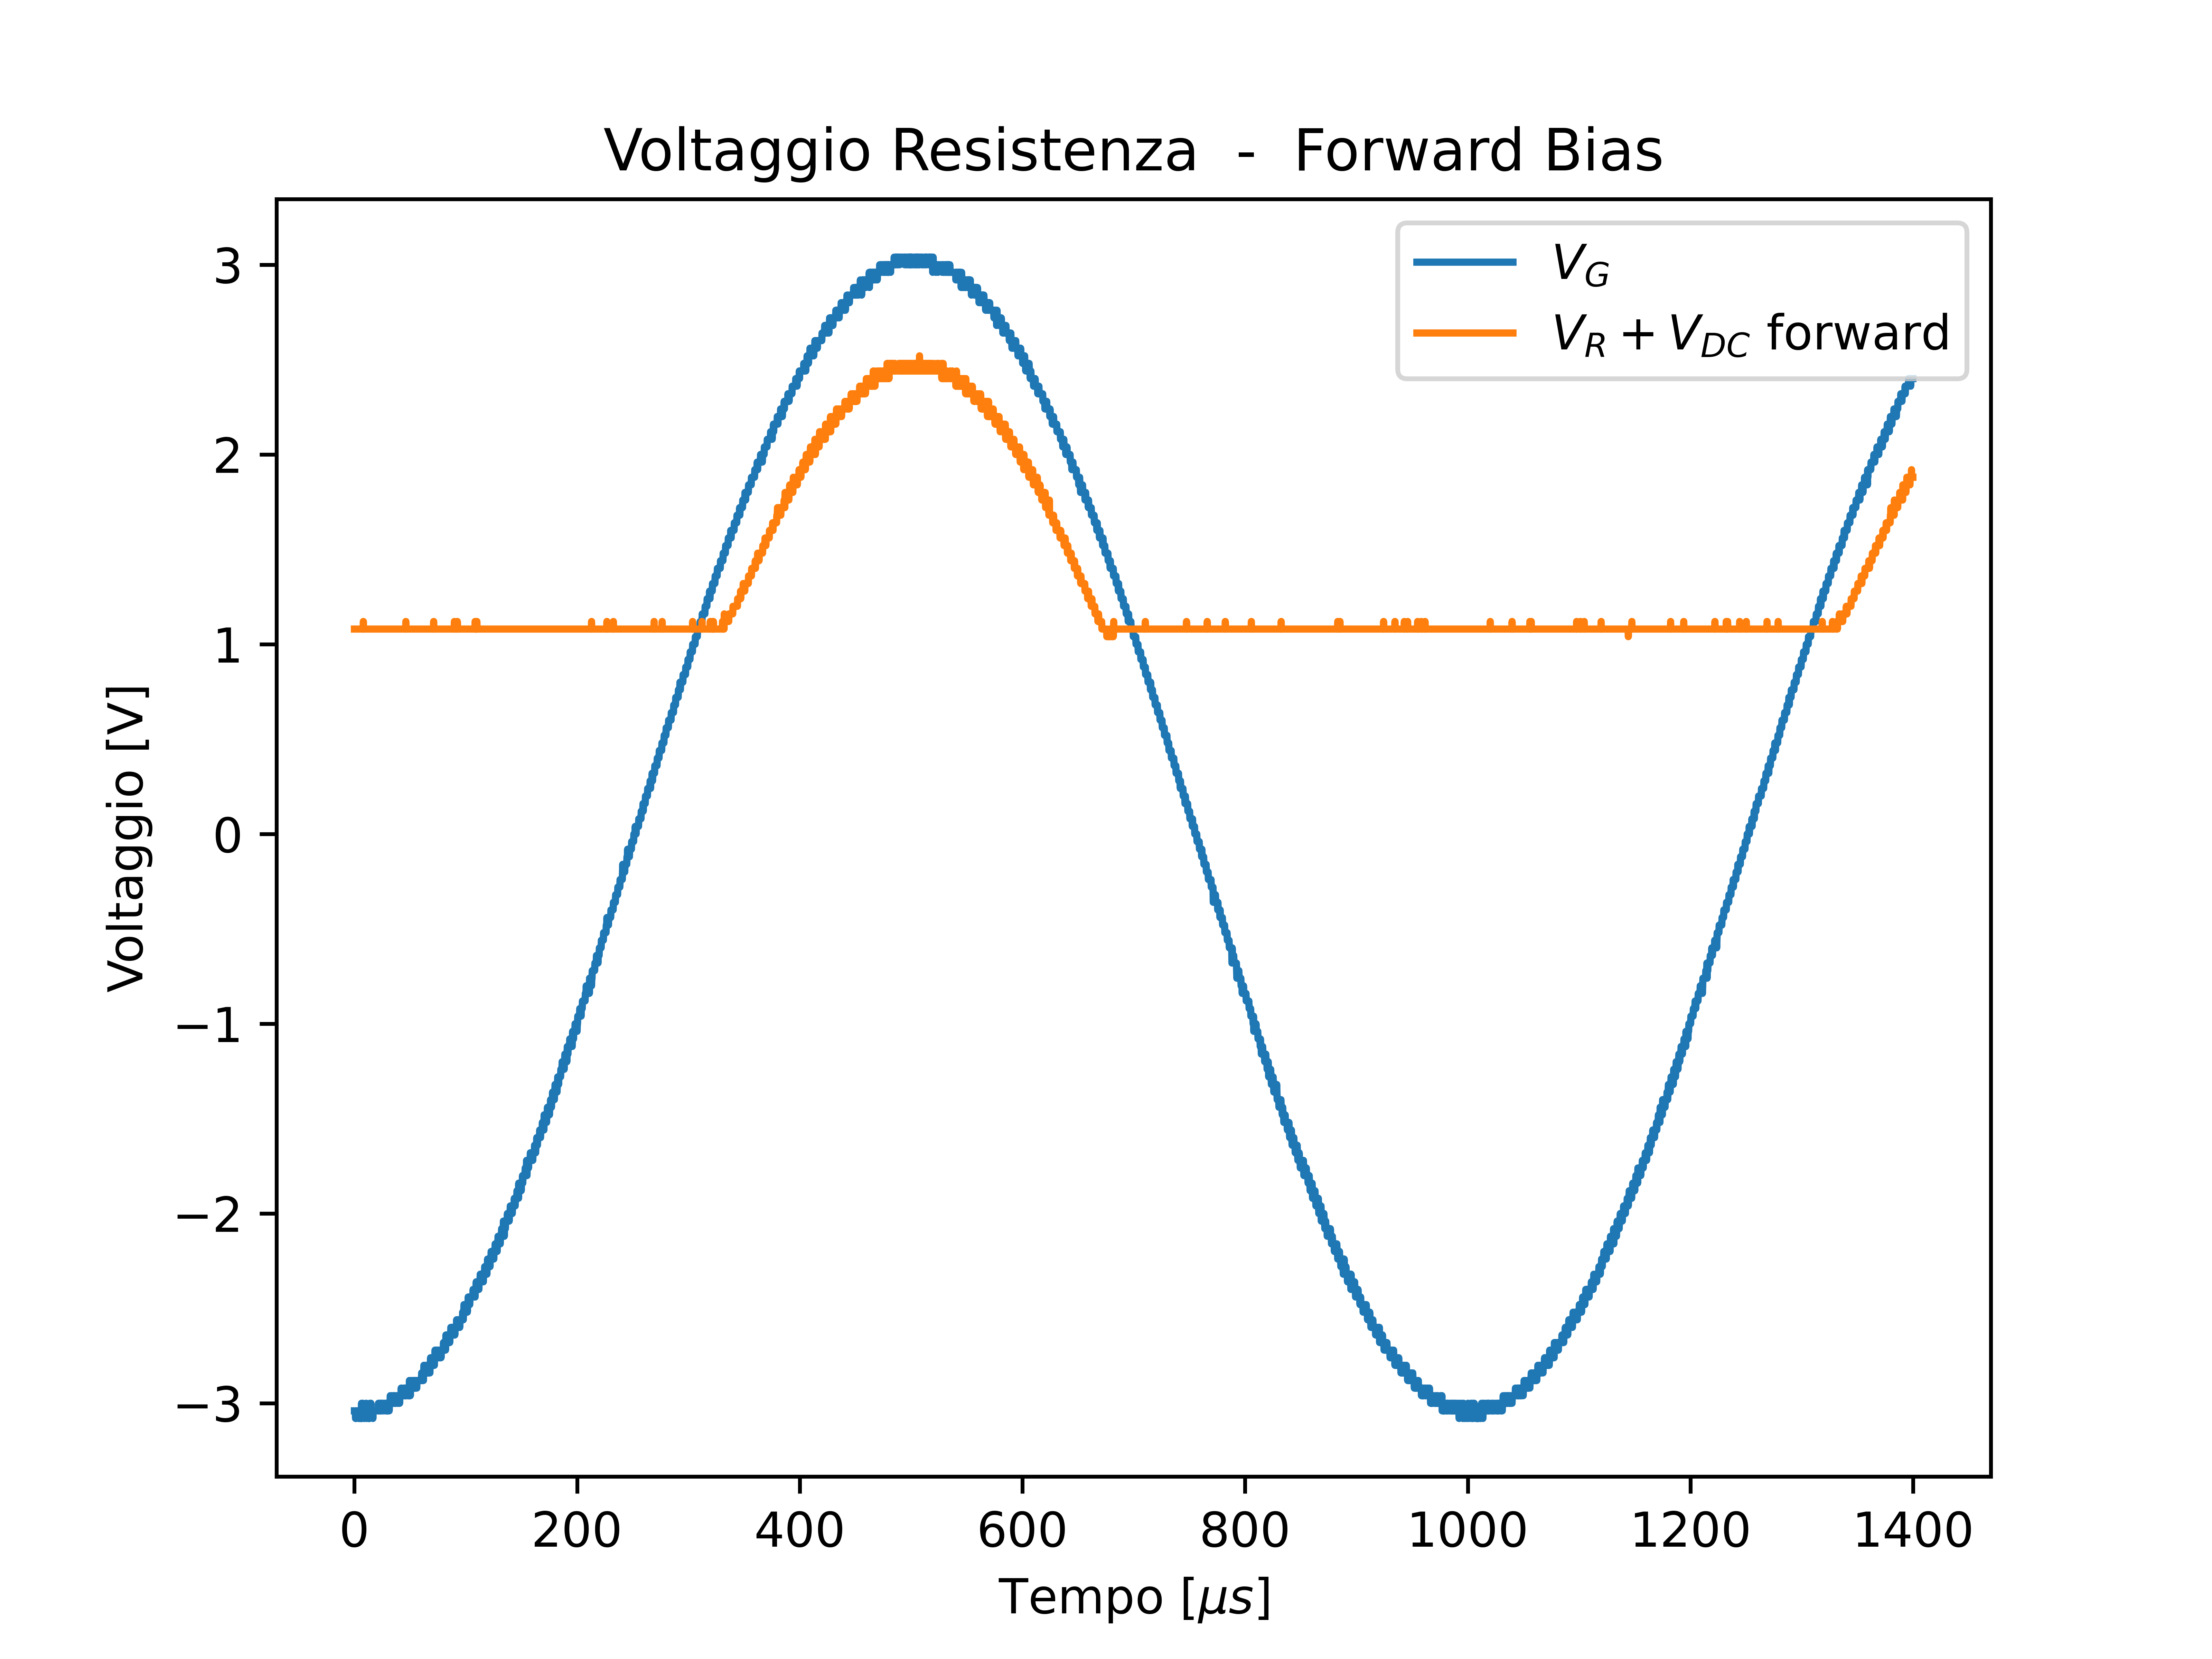
\includegraphics[width=1\textwidth]{Diodo 3.2.(4-5)/DC_V_R_Forward.png}
    \end{minipage}
    \label{3.2.5}
    \caption{Voltaggio ai capi di diodo e resistenza con $V_DC$ in reversed bias}
\end{figure}

\begin{figure}
    \centering
\begin{minipage}{0.475\textwidth}
\centering
\begin{circuitikz}[scale=0.7,american, voltage shift=0.5]
\ctikzset{bipoles/oscope/waveform=sin}
    \draw
(0,0)to [R,l_=$R$] (4,0)
    to [D,v=$V_d$](4,-3)
    to [short,-](0,-3)
    (0,0) to [oscope,v_=$V_g$](0,-3)
    (4,0) to [short,-](6,0)
    to [rmeterwa,t=V](6,-3)
    to [short,-](4,-3);
\end{circuitikz}
\end{minipage}
\hfill
\begin{minipage}{0.475\textwidth}
\centering
\begin{circuitikz}[scale=0.7,american, voltage shift=0.5]
\ctikzset{bipoles/oscope/waveform=sin}
    \draw
    (0,0)to [R,l_=$R$] (4,0)
    to [D,v=$V_d$](4,-1.5)
    to [battery2](4,-3)
    to [short,-](0,-3)
    (0,0) to [oscope,v_=$V_g$](0,-3)
    (4,0) to [short,-](6,0)
    to [rmeterwa,t=V](6,-3)
    to [short,-](4,-3);
    \draw (5,0) to [open,v=$V_{out}$] (5,-3);
\end{circuitikz}
\end{minipage}
\caption{Circuito raddrizzatore con e senza $V_{DC}$}
\label{fig: Raddrizzatore}
\end{figure}
\begin{figure}
    \centering
    \begin{minipage}{0.475\textwidth}
        \centering
        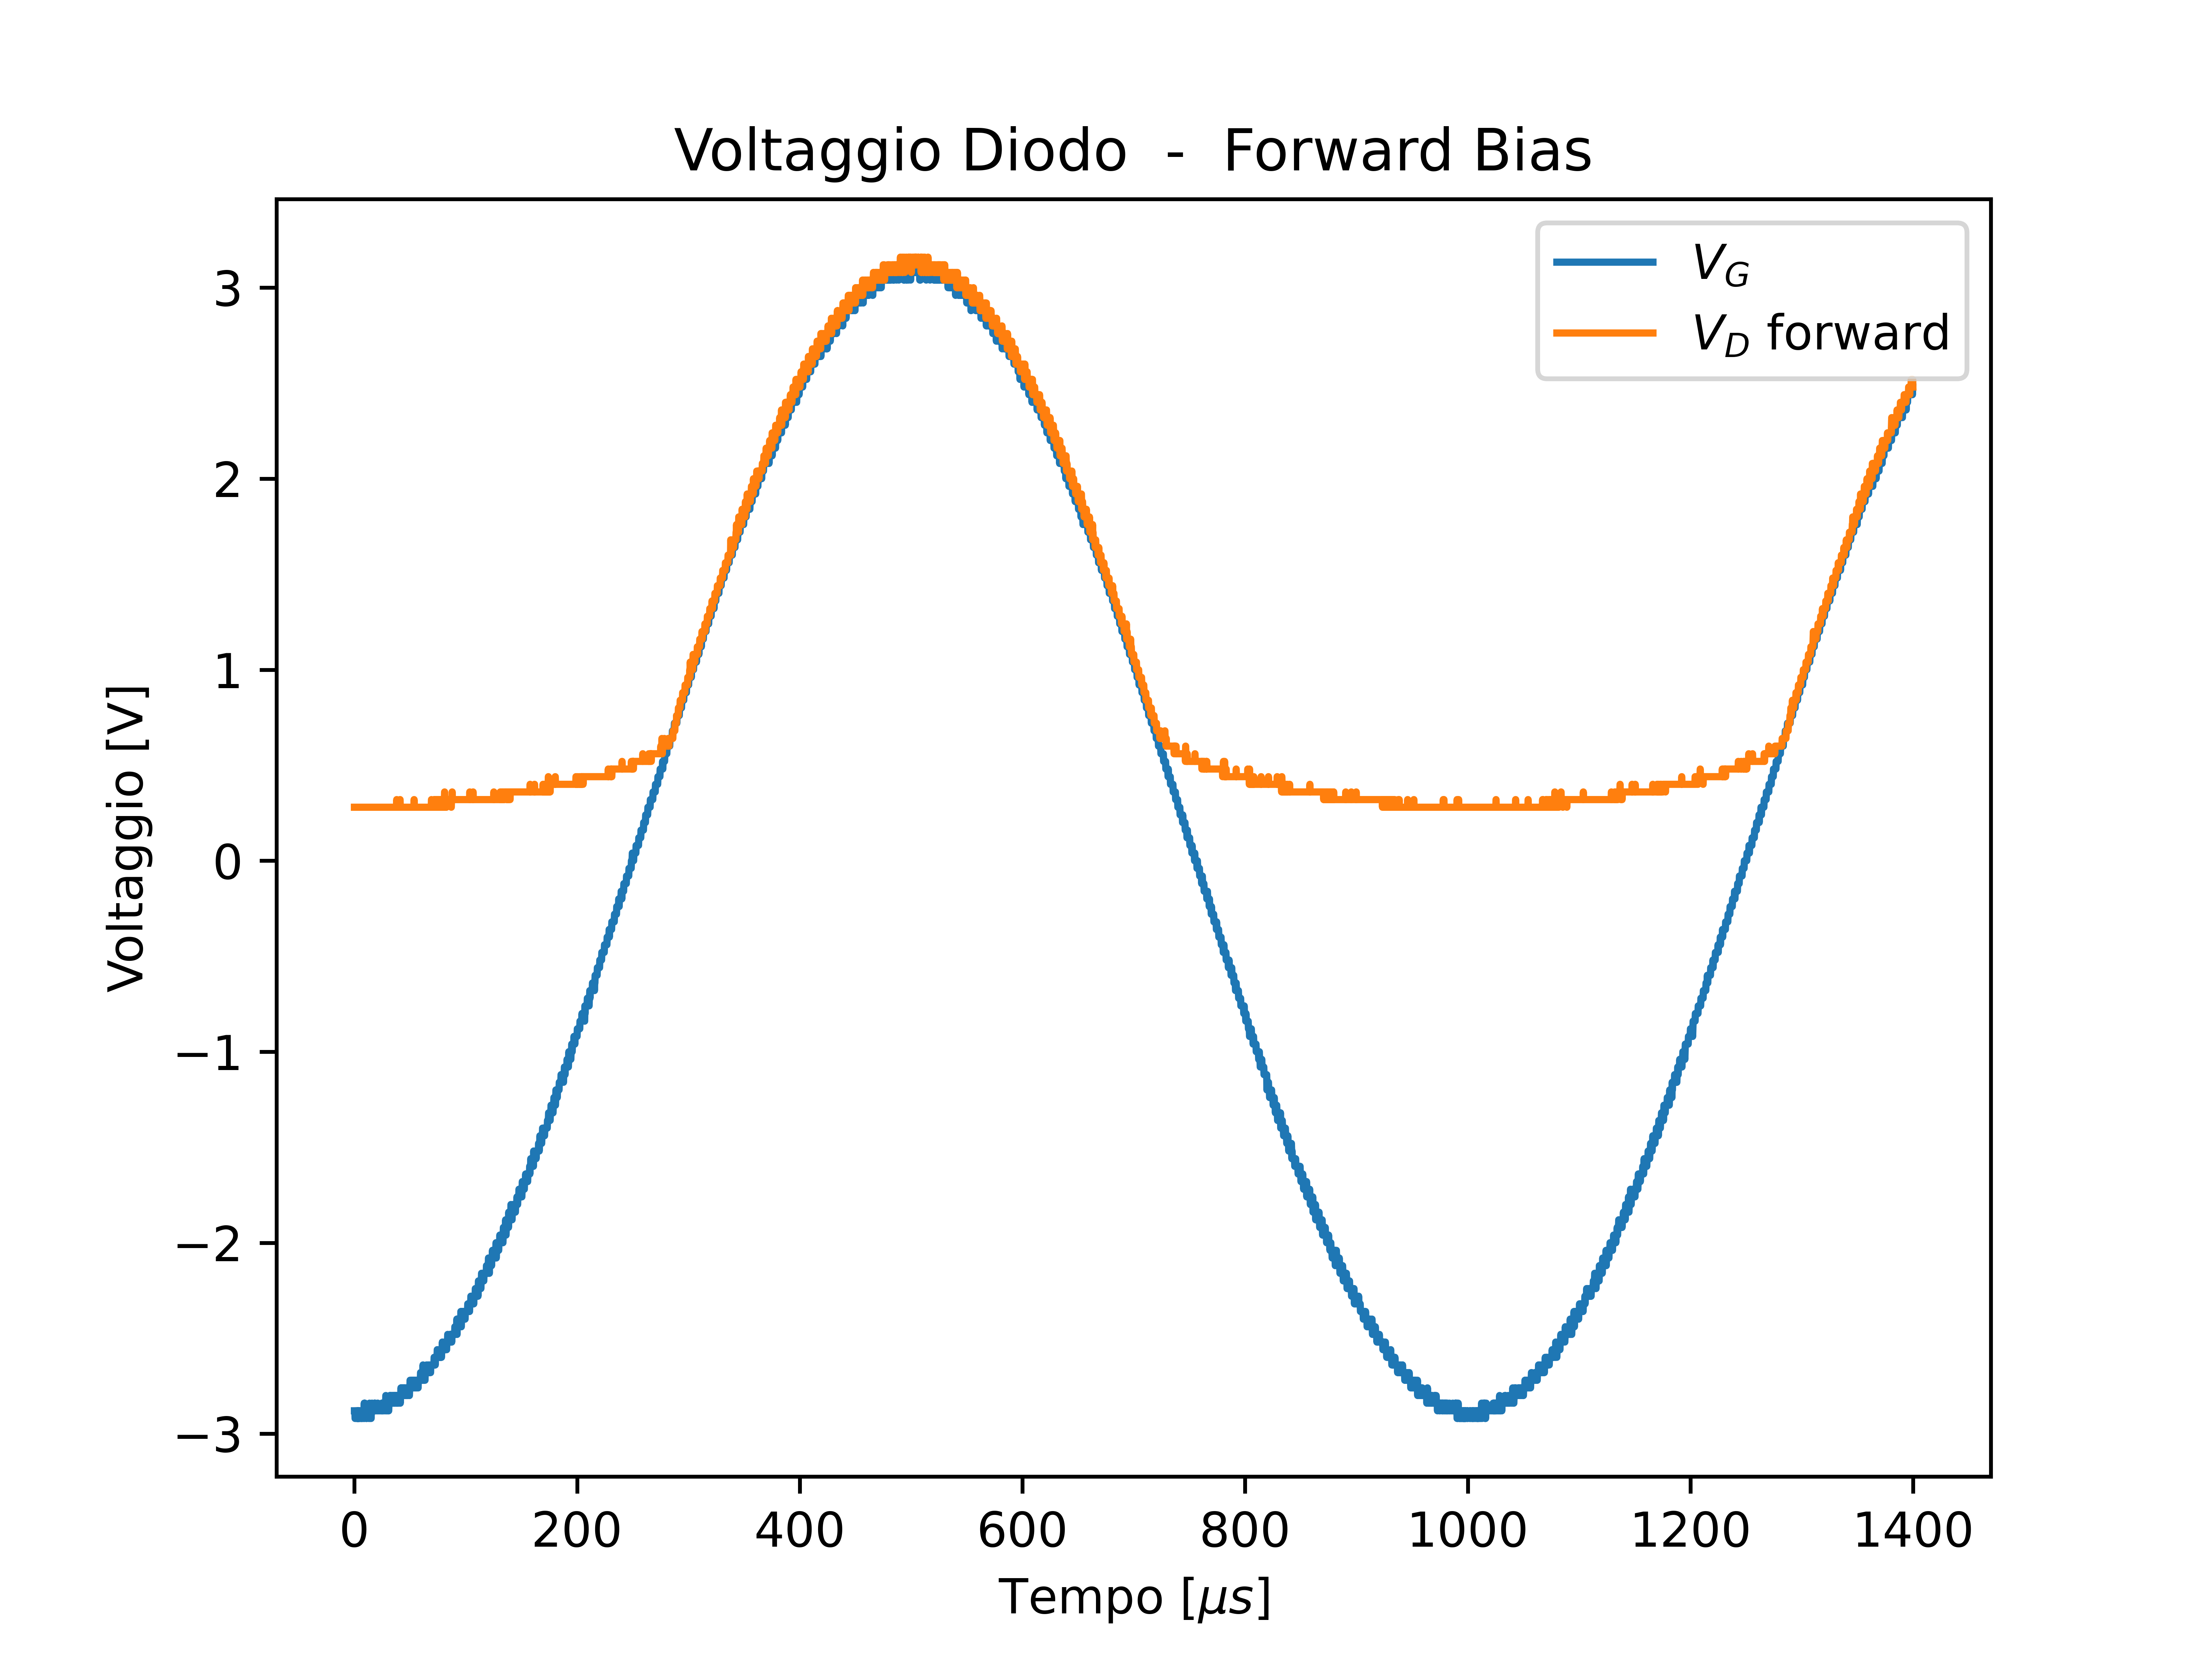
\includegraphics[width=1\textwidth]{Diodo 3.2.(4-5)/DC_V_D_Forward.png}
    \end{minipage}
    \hfill
    \begin{minipage}{0.475\textwidth}
        \centering
        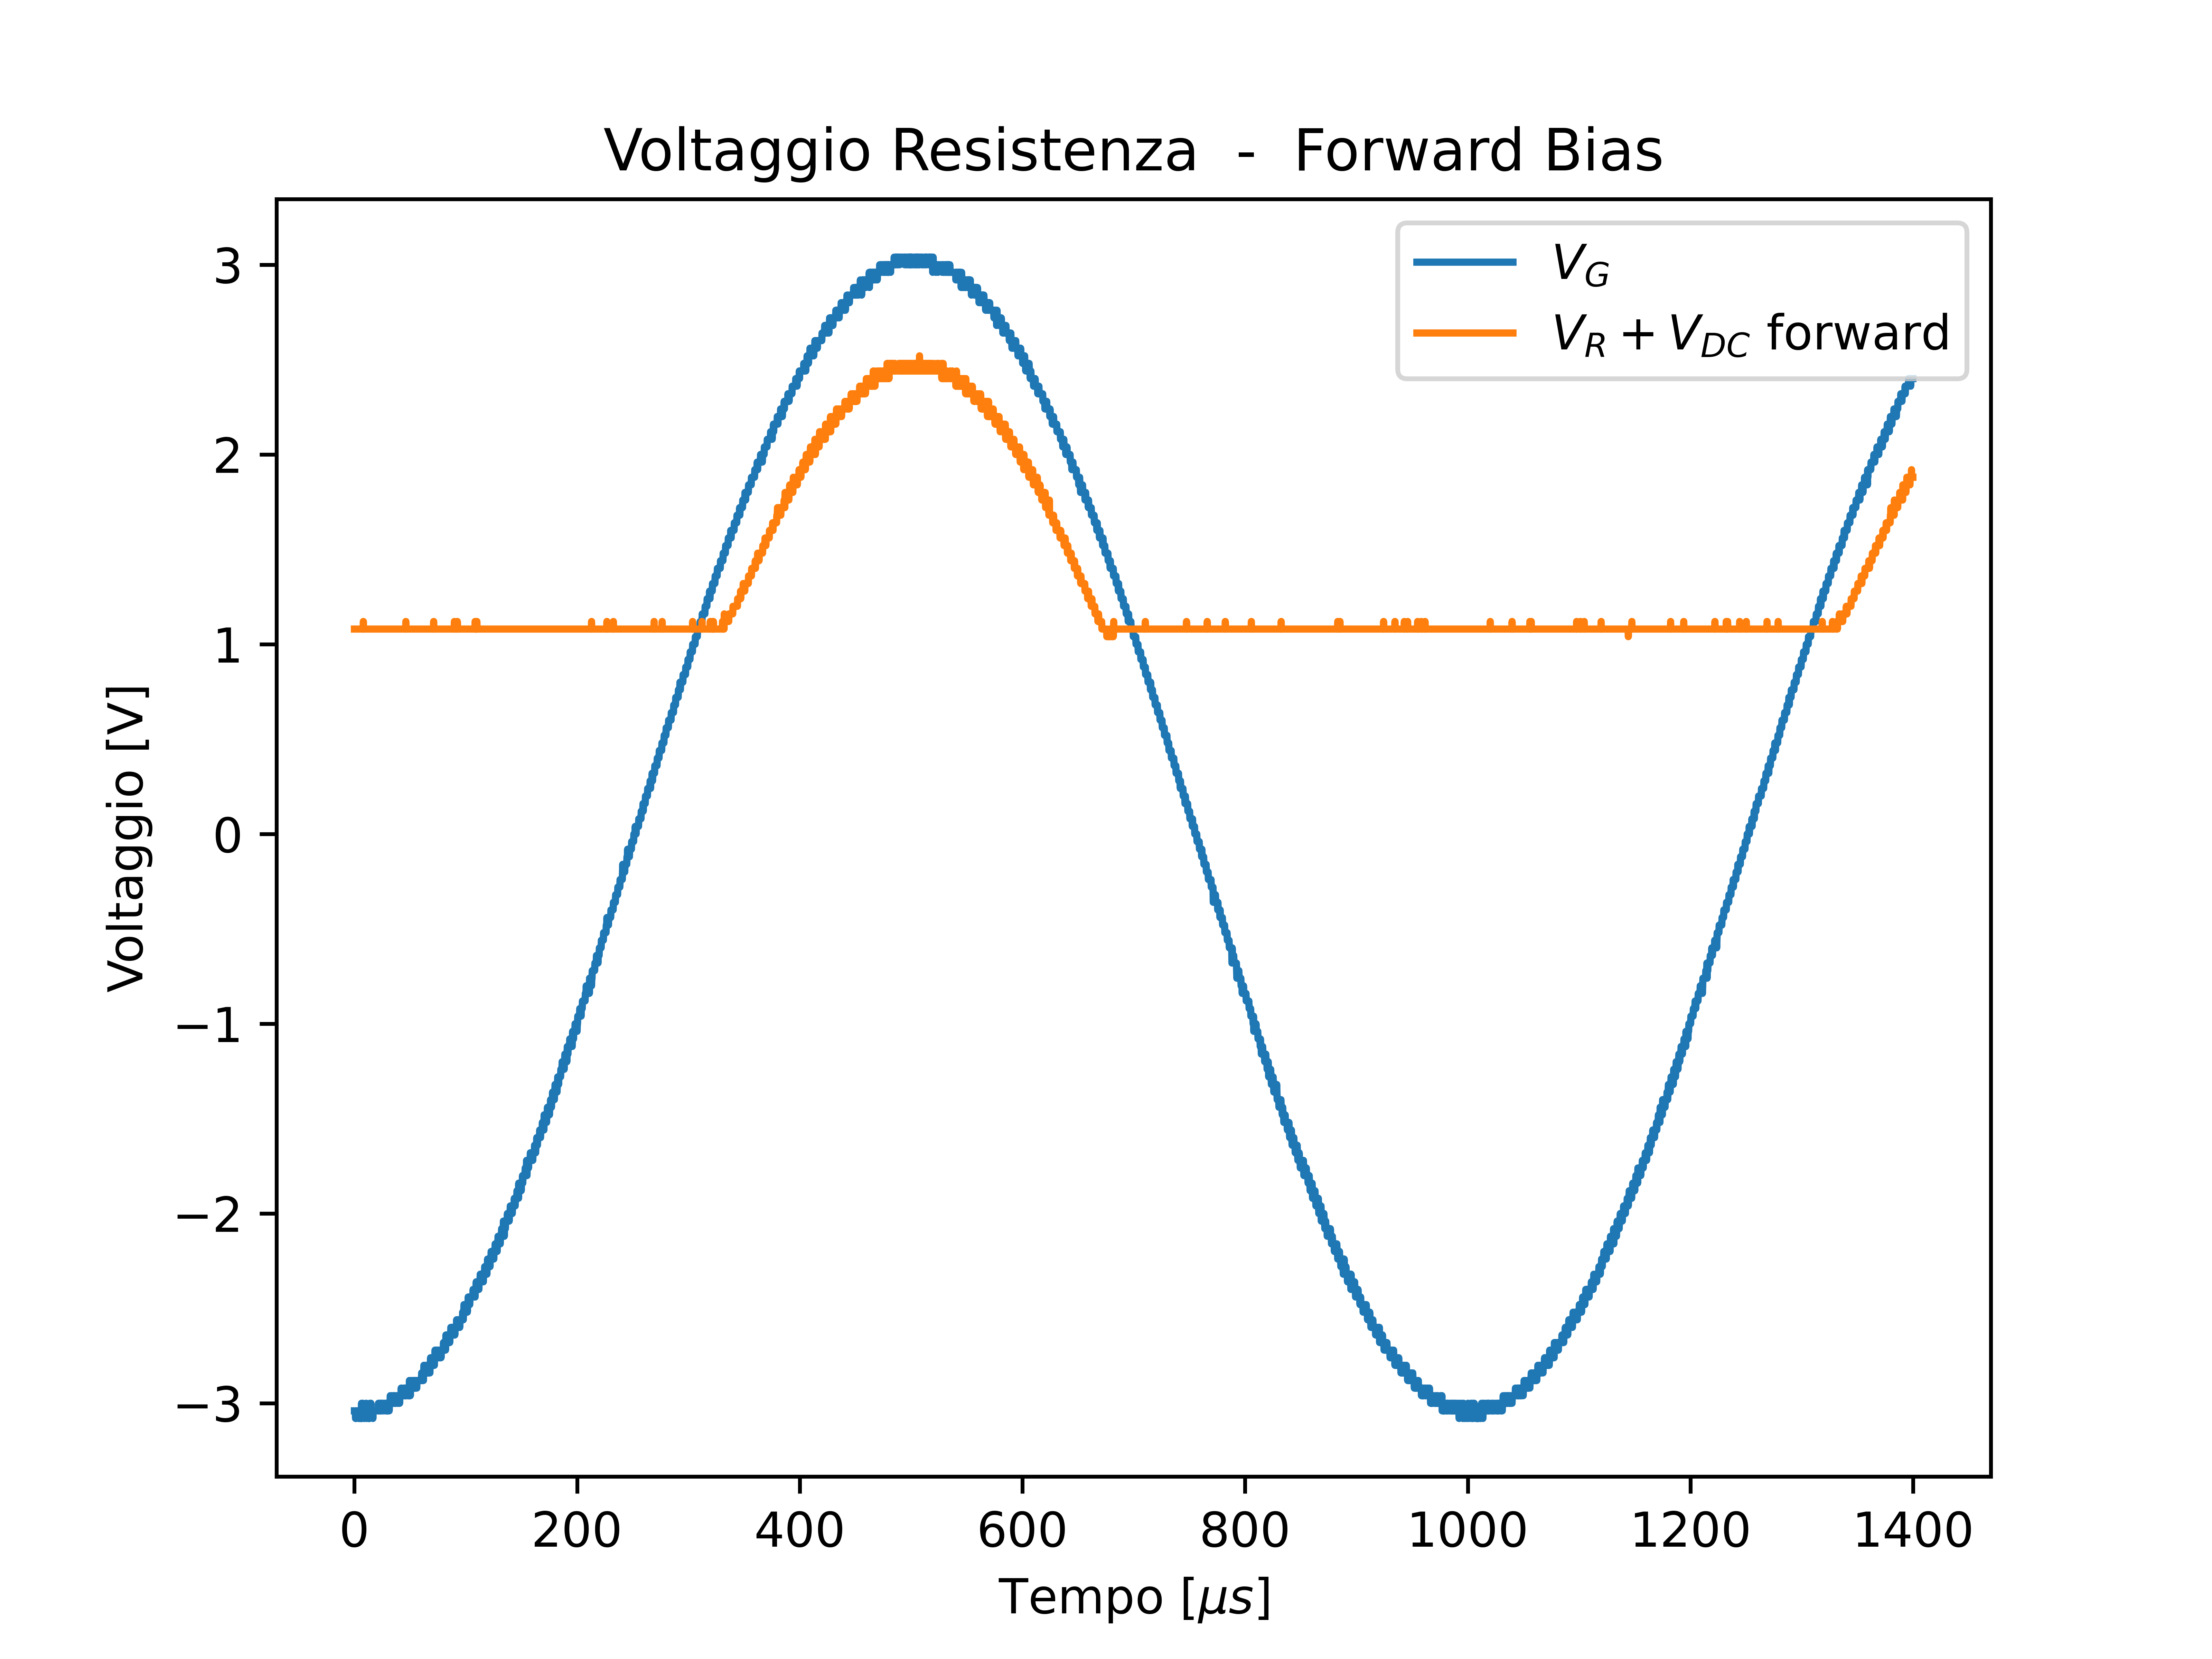
\includegraphics[width=1\textwidth]{Diodo 3.2.(4-5)/DC_V_R_Forward.png}
    \end{minipage}
    \caption{Voltaggio ai capi del diodo e della resistenza con $V_{DC}$ in forward bias}
    \label{3.2.4}
\end{figure}

\subsection{3.3}
In quest'esperienza si verifica il corretto funzionamento di un alimentatore a semionda il cui schema circuitale è quello riportato in figura \ref{fig: Stabilizzatore}. Lo scopo del circuito è quello di raddrizzare una tensione sinusoidale ad un suo valor medio, per fare ciò si sfrutta il carattere non lineare del diodo e la scarica del condensatore.
\subsubsection{3.3.1}
Il circuito è essenzialmente composto da un diodo e un filtro RC.\\
Lo scopo del circuito è quello di raddrizzare la tensione sinusoidale in ingresso e di mantenere un valore medio di tensione costante.\\
Per farlo si sfrutta il fatto che il diodo non permette il passaggio di corrente in verso opposto e che il condensatore si carica e si scarica in base alla tensione ai suoi capi.\\
In particolare, quando la tensione ai capi del condensatore è minore di quella in uscita dal generatore il diodo si polarizza direttamente e il condensatore si carica,
mentre quando la tensione ai capi del condensatore è maggiore di quella in uscita dal generatore il diodo si polarizza inversamente e il condensatore si scarica.\\
Si è quindi montato il circuito in figura \ref{fig: Stabilizzatore} con $C=10\unit{\nF},R_L=1\unit{\kohm}$ si è quindi variata la frequenza del generatore ($1\unit{\Hz},10\unit{Hz},100\unit{\Hz}$) e si è misurata la tensione ai capi del carico.\\
Il risultato è quello riportato in figura \ref{3.3.1}.
\subsubsection{3.3.1 (extra)}
Quando si sono misurate le tensioni di ronzio si è notato che per basse resistenze di carico la curva teorica non corrispondeva alle tensioni di ronzio misurate. Questo è un comportamento che ci saremmo dovuti aspettare dato che l'espressione della tensione di ronzio è stata trovata per $R_L \xrightarrow{}+\infty$. Tuttavia, nelle misure $R_L\xrightarrow{}0$! Pertanto è necessario riformulare la formula considerando, date le basse resistenze in gioco, anche la resistenza del generatore. Un' altro problema è che la tensione massima vista dal carico per basse resistenze non è più quella erogata dal generatore in quanto a quest'ultima viene tagliato il picco di tensione dal circuito R-Diodo creatosi (L'impedenza della capacità è praticamente nulla ad 1\unit{\kHz}). Per stimare la tensione di ripple supponiamo che la scarica del condensatore avvenga in un periodo, si ha pertanto:
\begin{equation}
    v_C(T)=V_{max}e^{-\frac{T}{\tau}}=V_{max}-\Delta V\Longrightarrow\Delta V=V_{max}\left[ 1-e^{-\frac{T}{\tau}}\right]
    \label{V_ripple}
\end{equation}
Si cerca quindi di stimare $V_{max}$, per fare ciò si considera il diodo in conduzione e la tensione erogata dal generatore massima nell'istante di tempo considerato. Il circuito da analizzare è pertanto quello in figura \ref{} ove si cerca di stimare la tensione ai capi del carico. Per fare ciò si usa Thevenin ai capi di $R_L$.
\begin{figure}
    \centering
    \caption{Caption}
    \label{fig:enter-label}
    \begin{circuitikz}[american, voltage shift=0.5]
    \draw
    (0,0) to [R,l=$R_g$](2,0)
    to [battery2,v=$V_\gamma$] (4,0)
    to [C](4,-3)
    to [short,-](0,-3)to [voltage source,v=$V_{max}$](0,0);
    \draw (4,0) to [short,-](6,0)
    to [R,l=$R_L$,v=$V_L$](6,-3)
    to [short,-](4,-3);
\end{circuitikz}
\end{figure}
Per il calcolo della tensione di Thevenin si utilizza il circuito in figura \ref{Thevenin equivalent} a destra.
Si ha quindi:
\begin{equation*}
    V_{max}-V_{\gamma}=R_g I+Z_C I\Longrightarrow I=\frac{V_{max}-V_{\gamma}}{R_g+Z_C}
\end{equation*}
Da cui:
\begin{equation*}
    V_{th}=V_{max} - R_g I - V_{\gamma}\Longrightarrow V_{th}=\frac{Z_C}{Z_C+R_g}(V_{max} - V_{\gamma})
\end{equation*}
Per il calcolo dell'impedenza di Thevenin si utilizza il circuito in figura \ref{Thevenin equivalent} a sinistra.
\begin{figure}
    \centering
    \begin{subfigure}[b]{0.4\textwidth}
        \begin{circuitikz}[american, voltage shift=0.5]
            \draw
            (0,0) to [R,l=$R_g$](4,0)
            to [C,l=$Z_C$](4,-3)--(0,-3)--(0,0);
            \draw
            (4,0) to [short,-*](5,0)
            to [open](5,-3)
            to [short,*-](4,-3);
        \end{circuitikz}
    \end{subfigure}
    \hfill
    \begin{subfigure}[b]{0.4\textwidth}
        \begin{circuitikz}[american, voltage shift=0.5]
            \draw
            (0,0) to [R,l=$R_g$](2,0)
            to [battery2,v=$V_\gamma$] (4,0)
            to [C,l_=$Z_C$](4,-3)--(0,-3)
            to [voltage source,v=$V_{max}$,invert](0,0);
            \draw
            (4,0) to [short,-*](5,0)
            to [open,v=$V_{th}$](5,-3)
            to [short,*-](4,-3);
        \end{circuitikz}
    \end{subfigure}
    \caption{Circuiti di Thevenin equivalenti}
    \centering
    \label{Thevenin equivalent}
\end{figure}
\begin{figure}
    \centering
        \begin{circuitikz}[american, voltage shift=0.5]
            \draw
            (0,0) to [generic,l=$Z_{th}$](3,0)
            to [R,l=$R_L$](3,-3)--(0,-3)
            to [voltage source,v=$V_{th}$,invert] (0,0);
        \end{circuitikz}
    \caption{Circuito equivalente}
    \label{Circuito equivalente}
\end{figure}
Da cui:
\begin{equation*}
    Z_{th}=\frac{R_gZ_C}{R_g+Z_C}
\end{equation*}
Il circuito equivalente è pertanto quello in figura \ref{Circuito equivalente}
Si trova quindi la tensione ai capi di $R_L$ che risulta essere pari a:
\begin{equation}
    V_L=\frac{R_L}{Z_{th}+R_L}V_{th}
    \label{V_L raddr}
\end{equation}
Se pertanto si inserisce $V_L$ nell'equazione \ref{V_L raddr} all'interno dell'equazione \ref{V_ripple} al posto di $V_{max}$ si ottiene l'equazione:
\begin{equation}
    \Delta V = \frac{R_L}{Z_{th}+R_L}V_{th}\left[ 1-e^{-\frac{T}{\tau}}\right]
    \label{V_ripple_mod}
\end{equation}
Si sono quindi misurati sperimentalmente le tensioni di ronzio tramite l'oscilloscopio e si è confrontato con l'equazione teorica \ref{V_ripple_mod}. Il risultato è quello ottenuto in figura \ref{Figura ripple}
\begin{figure}
    \centering
    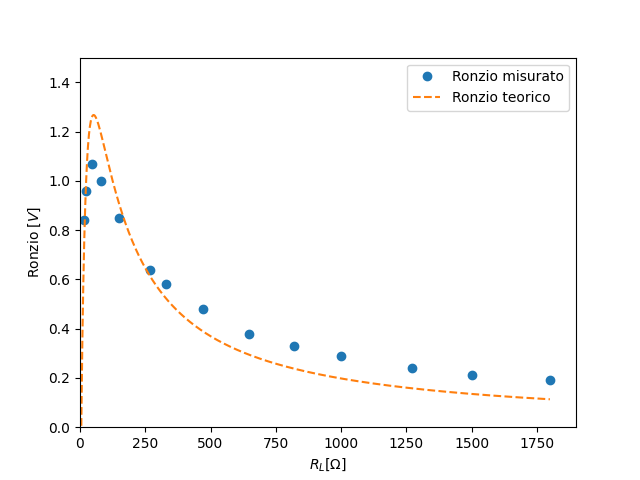
\includegraphics[scale=0.7]{Figuraripple.png}
    \caption{Caption}
    \label{Figura ripple}
\end{figure}
\begin{figure}
\centering
\begin{circuitikz}[american, voltage shift=0.5]
\ctikzset{bipoles/oscope/waveform=sin}
    \draw
    (0,0)to [D] (4,0)
    to [C](4,-3)
    to [short,-](0,-3)to [oscope,v^<=$V_g$](0,0);
    \draw (4,0) to [short,-](6,0)
    to [R,l=$R_L$,v=$V_L$](6,-3)
    to [short,-](4,-3);
    \draw (6,0) -- (8,0)
    to [rmeterwa,t=V] (8,-3) -- (6,-3);
\end{circuitikz}
   \caption{Circuito stabilizzatore}
    \label{fig: Stabilizzatore}
\end{figure}

\subsection{3.4}
In quest'esperienza si è studiato il comportamento di un alimentatore stabilizzzato realizzato con un diodo Zener.\\
Lo schema circuitale è quello in figura \ref{fig: Stabilizzatore Zener}.\\
Il principio di funzionamento è basato sul fatto che il diodo Zener polarizzato inversamente, una volta raggiunta la tensione di Zener, mantiene costante la tensione ai suoi capi, sfruttando l'effetto Zener.\\
Si è quindi montato il circuito in figura \ref{fig: Stabilizzatore Zener} con $V_g=10\unit{\V}$ alla frequenza di $1\unit{\kHz}$.
Si è scelto una $R_z=$
\begin{figure}
    \centering
    \begin{circuitikz}[american, voltage shift=0.5]
        \draw
        (0,0) to [voltage source,v^=$V_g$,invert](0,3)
        to [R,l=$R_z$](4,3)
        to [zzDo,invert](4,0)
        to [short,-](0,0);
        \draw (4,3) to [short,-](6,3)
        to [R,l=$R_L$,v^=$V_{out}$](6,0)
        to [short,-](4,0);
    \end{circuitikz}
    \caption{Circuito stabilizzatore Zener}
    \label{Stabilizzatore Zener}
\end{figure}